\documentclass{report}
\usepackage{amsmath, amssymb, amsthm, amsfonts}
\usepackage{mathrsfs, bm, mathtools}
\usepackage{graphicx}
\usepackage{listings}

\newcommand{\son}{\mathbf{N}}
\newcommand{\sor}{\mathbf{R}}
\newcommand{\soi}{\mathbf{Z}}
\newcommand{\soc}{\mathbf{C}}
\newcommand{\bs}[1]{\boldsymbol{#1}}

\DeclareMathOperator{\card}{card}
\DeclareMathOperator{\rank}{rank}
\DeclareMathOperator{\nullity}{nullity}
\DeclareMathOperator{\ev}{E}
\DeclareMathOperator{\var}{var}
\DeclareMathOperator{\cov}{cov}
\DeclareMathOperator{\tr}{tr}
\DeclareMathOperator{\diag}{diag}
\DeclareMathOperator*{\argmin}{arg\,min}
\DeclareMathOperator*{\argmax}{arg\,max}
\DeclareMathOperator{\kl}{KL}

\DeclarePairedDelimiter\abs{\lvert}{\rvert}
\DeclarePairedDelimiter\norm{\lVert}{\rVert}

\lstset{basicstyle=\ttfamily\footnotesize}

\title{Pattern Recognition and Machine Learning \\ Solutions and Notes}
\author{Amey Joshi}
\date{24-Dec-2019}
\begin{document}
\graphicspath{ {./images/} }
\pagenumbering{Alph}
\begin{titlepage}
\maketitle
\thispagestyle{empty}
\end{titlepage}

\pagenumbering{roman}		
\tableofcontents
\thispagestyle{empty}

%\include{abstract}

\pagenumbering{arabic}	
\numberwithin{equation}{section}

\theoremstyle{plain}
\newtheorem{thm}{Theorem}[section]

\theoremstyle{plain}
\newtheorem{prop}{Proposition}[section]

\theoremstyle{plain}
\newtheorem{lem}{Lemma}[section]

\theoremstyle{plain}
\newtheorem{corr}{Corollary}[section]

\theoremstyle{definition}
\newtheorem{defn}{Definition}[section]

\theoremstyle{remark}
\newtheorem*{rem}{Remark}

\chapter{Introduction}\label{c1}
\section{Notation and definitions}\label{c1s1}
We will follow the contemporary mathematical style of using unadorned symbols for vectors and
matrices. The nature of a symbol will be determined by its definition and not appearance. For
example, $x$ could be a real number or a point in $\sor^n$ depending on the context. Random
variables will be denoted by capital letters and their realizations by small letters.

A matrix with entries $a_{ij}$ will sometimes be denoted by $((a_{ij}))$.

If $f$ is a function of $n$ variables, $x_1, \ldots, x_n$ then its gradient is defined as
\begin{equation}\label{c1s1e1}
Df := \left(\frac{\partial f}{\partial x_1}, \ldots, \frac{\partial f}{\partial x_n}\right).
\end{equation}
The hessian of $f$ is
\begin{equation}\label{c1s1e2}
(D^2 f)_{ij} := \frac{\partial^2 f}{\partial x_i \partial x_j}.
\end{equation}

The integrals are almost always definite. If the limits are not specified then it is usually safe
to conclude that the integral is over $\sor^n$ for an appropriate $n$.

\section{Bayesian curve fitting}\label{c1s2}
The problem consists of using the data $\{(x_i, t_i) : 1 \le i \le n\}$ to find the value
of $t$ when a new $x$ is given. We shall fit the data using the polynomial
\begin{equation}\label{c1s2e1}
y(x, w) = \sum_{i=0}^M w_i x^i.
\end{equation}
The polynomial coefficients $w_0, \ldots, w_M$ can be considered to be components of a 
vector $w \in \sor^M$. We assume that for a given value of $x_i$, the target $t_i$ has a 
gaussian distribution with mean $y(x, w)$ and precision $\beta$ (or variance $\beta^{-1}$).
Thus,
\begin{equation}\label{c1s2e2}
p(t_i | x_i, w, \beta) = \mathcal{N}(t | y(x_i, w), \beta^{-1/2}).
\end{equation}
We will use the training data $\{(x_i, t_i): 1 \le i \le N\}$ to estimate the values of $w$
and $\beta$ using maximizing the likelihood function. If the data are assumed to be drawn
independently from the distribution of equation \eqref{c1s2e2} then the likelihood function
is
\[
p(t | x, w, \beta) = \prod_{i=1}^N p(t_i | x_i, w, \beta) = \prod_{i=1}^N \mathcal{N}(y(x_i, w), \beta^{-1/2})
\]
where $x, t \in \sor^n$, $w \in \sor^{M+1}$ and $y$ is given by \eqref{c1s2e1}. The log-likelihood
function is
\begin{equation}\label{c1s2e3}
\ln p(t|x,w,\beta) = -\frac{\beta}{2}\sum_{i=1}^N(y(x_i, w) - t_i)^2 + \frac{N}{2}\ln\beta - \frac{N}{2}\ln(2\pi).
\end{equation}
Maximizing $\ln p$ with respect to $w$ is the same as minimizing the quantity,
\begin{equation}\label{c1s2e4}
\sum_{i=1}^N(y(x_i, w) - t_i)^2.
\end{equation}
This quantity is the sum of squares of residuals and the problem of finding optimal $w$ reduces
to that of ordinary least squares regression. In order to find $\beta$ that maximizes $\ln p$
we differentiate the equation with respect to $\beta$ to get
\[
\frac{\partial}{\partial\beta}\ln p(t|x,w,\beta) = -\frac{1}{2}\sum_{i=1}^N(y(x_i, w) - t_i)^2 + \frac{N}{2\beta}
\]
The derivative vanishes when $\beta = \beta_{ML}$, where
\begin{equation}\label{c1s2e5}
\frac{1}{\beta_{ML}} = \frac{1}{N}\sum_{i=1}^N(y(x_i, w) - t_i)^2.
\end{equation}
If we are now given a new $x$, say $x_{N+1}$ then the corresponding target value $t_{N+1}$ has
a distribution
\[
p(t_{N+1} | x_{N+1}, w_{ML}, \beta_{ML}) = \mathcal{N}(t_{N+1}| y(x_{N+1}, w_{ML}), \beta_{ML}^{-1}).
\]

We now choose a prior distribution for $w$. Let it be a gaussian with mean zero and variance-covariance
matrix $\alpha^{-1}I$, where $I$ is an $(M+1) \times (M+1)$ identity matrix. Thus,
\begin{equation}\label{c1s2e6}
p(w|\alpha) = \mathcal{N}(w|0, \alpha^{-1}I) = \left(\frac{\alpha}{2\pi}\right)^{(M+1)/2}\exp\left(-\frac{\alpha}{2}w^Tw\right).
\end{equation}
The posterior distribution for $w$ given $(x_i, t_i), \alpha, \beta$ is
\begin{equation}\label{c1s2e7}
p(w|x, t, \alpha, \beta) \propto p(t|x,w,\beta)p(w|\alpha).
\end{equation}
We can now find $w$ suitable for the data by maximizing the right hand side. The posterior probability
on the right hand side is conditioned on the data $(x, t)$, the hyperparameter $\alpha$ and the maximum
likelihood estimate $\beta$. Taking a logarithm of both sides of equation \eqref{c1s2e7},
\[
\ln p(w|x,t,\alpha,\beta) = \ln p(t|x,w,\beta) + \ln p(w|\alpha) + \ln K,
\]
where $K$ is the constant of proportionality in \eqref{c1s2e7}. From equations \eqref{c1s2e3} and
\eqref{c1s2e6} we get
\[
\ln p(w|x,t,\alpha,\beta) = -\frac{\beta}{2}\sum_{i=1}^N(y(x_i, w) - t_i)^2 + \frac{N}{2}\ln\beta - \frac{N}{2}\ln(2\pi) - \frac{\alpha}{2}w^Tw + \ln K.
\]
Maximizing $\ln p(w|x,t,\alpha,\beta)$ with respect to $w$ is equivalent to minimizing the function
\[
\frac{\beta}{2}\sum_{i=1}^N(y(x_i, w) - t_i)^2 + \frac{\alpha}{2}w^Tw.
\]
This expression is the regularized least square error of equation (1.4) of the book. Equations (1.68) to (1.72)
will be derived in chapter 3.

\section{Problems}\label{c1p}
\begin{enumerate}
\item In this problem, $w = (w_0, \ldots, w_M) \in \sor^{M+1}$, $x, y \in \sor$. Likewise, the $n$
observations $y_1, \ldots, y_n$ for each one of $x_1, \ldots, x_n$ are also real numbers. $y$
is modelled as a polynomial in $x$. That is,
\begin{equation}\label{c1pe1}
y = y(x, w) = \sum_{i=0}^Mw_ix^i.
\end{equation}
The model error is given by
\begin{equation}\label{c1pe2}
E(w) = \frac{1}{2}\sum_{j=1}^N \left(y(x_j, w) - t_j\right)^2,
\end{equation}
where $t_j$ is the true value of $y$ at $x_j$. The goal of the exercise is to choose $w$ such 
that for a given set of observations $(x_j, t_j)$, $E$ is minimal. Therefore, we find the
gradient of $E$,
\[
DE = \sum_{j=1}^N\left(y(x_j, w) - t_j\right)Dy.
\]
The gradient of $y$ with respect to $w$ is
\[
Dy = \sum_{i=0}^M x^i,
\]
so that
\[
DE = \sum_{j=1}^N\left(y(x_j, w) - t_j\right)\sum_{i=0}^M x_j^i.
\]
The condition for an extremum is $DE = 0$. The vector $DE$ is zero if and only if each one
of its components is zero.
\[
\sum_{j=1}^N\left(\sum_{k=0}^M w_k x_j^{k+i} - t_jx_j^i\right) = 0, \forall i = 0, \ldots, M
\]
We can simplify it as
\[
\sum_{k=0}^M \sum_{j=1}^N w_k x_j^{k+i} = \sum_{i=0}^M\sum_{j=1}^N t_jx_j^i.
\]
Let,
\begin{eqnarray*}
T_i &=& \sum_{j=1}^N t_jx_j^i \\
A_{ik} &=& \sum_{j=1}^N x_j^{k+i}
\end{eqnarray*}
so that the condition from an extremum becomes
\[
\sum_{k=0}^M A_{ik}w_k = T_i
\]

\item The regularized error function is
\begin{equation}\label{c1pe3}
E(w) = \frac{1}{2}\sum_{j=1}^N \left(y(x_j, w) - t_j\right)^2 + \frac{\lambda}{2}\norm{w}^2.
\end{equation}
Its gradient is
\[
DE = \sum_{j=1}^N\left(y(x_j, w) - t_j\right)Dy + \lambda w,
\]
where we have used the fact that 
\[
D\norm{w}^2 = \left(\frac{\partial}{\partial w_0}\sum_{i=0}^M w_i^2, \ldots, \frac{\partial}{\partial w_M}\sum_{i=0}^M w_i^2\right) = 2w.
\]
The vector $DE = 0$ if and only if all its components are zero. Therefore,
\[
\sum_{j=1}^N\left(\sum_{k=0}^M w_k x_j^{k+i} - t_jx_j^i\right) + \lambda w_i = 0, \forall i = 0, \ldots, M
\]
Using the definitions of $A_{ik}$ and $T_i$ introduced in the previous problem, the condition
for extremum becimes
\[
\sum_{k=0}^M A_{ik}w_k = T_i - \lambda w_i.
\]

\item We are given that $p(r) = 0.2, p(b) = 0.2, p(b) = 0.6$. The conditional probabilities are
$p(a|r) = 0.3, p(o|r) = 0.4, p(l|r) = 0.3$, $p(a|b) = 0.5, p(o|b) = 0.5$ and $p(a|g) = 0.3, p(o|g)
= 0.3, p(l|g) = 0.6$.

Now, 
\[
p(a) = p(a|r)p(r) + p(a|b)p(b) + p(a|g)p(g) = 0.34.
\]

If the selected fruit is orange, the probability that it came from the green box is $p(g|o)$. Using
Bayes theorem,
\[
p(g|o) = \frac{p(g, o)}{p(o)} = \frac{p(o|g)p(g)}{p(o)}.
\]
The denominator is calculated as
\[
p(o) = p(o|r)p(r) + p(o|b)p(b) + p(o|g)p(g) = 0.36
\]
Therefore,
\[
p(g|o) = \frac{0.3 \times 0.6}{0.36} = 0.5.
\]

\item Consider equation (1.27) of the book. Instead of writing it with modulus, we write it as
\[
p_y(y) = \pm p_x(g(y))g^\prime(y),
\]
where we chose the sign to make $p_y \ge 0$ for all $y$. The extremum of this function is found
using the relation
\begin{equation}\label{c1pe4}
p_y^\prime(y) = \pm\left(\frac{dp_x}{dg}\left(g^\prime(y)\right)^2 + p_x(g(y))g^{\prime\prime}(y)\right)
\end{equation}
and equating it to zero. If instead of a probability density, we had an ordinary
function $h(y) = f(g(y))$. Then $h^\prime(y) = df/dg g^\prime(y)$ and the condition for extremum
would be $df/dg = 0$ if $g^\prime(y) \ne 0$. The value of $y$ obtained using this relation
is related to the $x$ found using $f^\prime(x) = 0$ is precisely $x = g(y)$. However, it
is not so because of the second term on the right hand side of equation \eqref{c1pe4}.

However, if $g$ is a linear function of $y$ then its second derivative vanishes and the two
equations become similar.

\item We start with the definition $\var(f) = \ev(f(x) - \ev(f(x)))^2 = \ev(f^2(x) - 2f(x)\ev(f(x)) + (\ev(f(x)))^2)
= \ev(f^2(x)) - 2\ev(f(x))\ev(f(x)) + (\ev(f(x))^2) = \ev(f^2(x)) - (\ev(f(x)))^2$, where we 
have used the fact that $\ev(x)$ is a constant and $\ev1(ax) = a\ev(x)$ for any constant $a$.

\item The covariance of two random variables $X$ and $Y$ is given by $\cov(X, Y) = \ev(XY) - \ev(X)\ev(Y)$.
If $p$ is the joint probability density of $X$ and $Y$ and if $p_X$ and $p_Y$ are the respective marginal 
probability densities then,
\begin{eqnarray*}
\ev(XY) &=& \iint p(X, Y)Xy dXdy \\
\ev(X)  &=& \int p_X(X) X dX \\
\ev(Y)  &=& \int p_Y(Y) y dy
\end{eqnarray*}
If $X$ and $Y$ are independent $p(X, Y) = p_{X|Y}(X|Y)p_Y(Y) = p_X(X)p_Y(Y)$ and the $\ev(XY)$ simplifies
to
\[
\ev(XY) = \int p_X(X)XdX \int p_Y(Y)ydy.
\]
The covariance of independent random variables thus vanishes.

\item The proof of normality of the gaussian distribution depends on the integral of $\exp(-ax^2)$
over the real line. Here $a$ is a real constant and $x$ a real variable. Let
\[
I = \int_\sor e^{-ax^2}dx = \int_\sor e^{-ay^2}dy.
\]
Therefore,
\[
I^2 = \iint_{\sor\times\sor}e^{-a(x^2+y^2)}dxdy.
\]
Change the coordinates from $(x, y)$ to $(r, \theta)$, where $x = r\cos\theta$ and $y = r\sin\theta$.
The jacobian of transformation is $r$ so that
\[
I^2 = \int_0^\infty\int_0^{2\pi}e^{-ar^2}rdrd\theta = 2\pi\int_0^\infty e^{-ar^2}rdr.
\]
Introduce the variable $s = r^2$ so that $ds = 2rdr$ and hence,
\[
I^2 = \pi\int_0^\infty e^{-as}ds = \frac{\pi}{a}
\]
so that
\begin{equation}\label{c1pe5}
\int_\sor e^{-ax^2}dx = \sqrt{\frac{\pi}{a}}.
\end{equation}
The normal density is
\[
\mathcal{N}(x|\mu,\sigma) = \frac{1}{\sqrt{2\pi\sigma^2}}\exp\left(-\frac{(x - \mu)^2}{2\sigma^2}\right)
\]
so that
\[
\int_\sor\mathcal{N}(x|\mu,\sigma)dx = \frac{1}{\sqrt{2\pi\sigma^2}}\int_\sor\exp\left(-\frac{(x - \mu)^2}{2\sigma^2}\right)dx.
\]
Introduce the variable $u = (x - \mu)/(\sigma\sqrt{2})$ so that $dx = \sigma\sqrt{2}du$ and the limits of the integral
remain unchanged. Thus,
\[
\int_\sor\mathcal{N}(x|\mu,\sigma)dx = \frac{1}{\sqrt{\pi}}\int_\sor e^{-u^2}du = 1.
\]

\item Let $X$ be a random variable with distribution $\mathcal{N}(x|\mu,\sigma)$. Then its expectation
is
\[
\ev(X) = \int_\sor\mathcal{N}(x|\mu,\sigma)xdx.
\]
Introduce the variable
\begin{equation}\label{c1pe6}
u = \frac{x - \mu}{\sigma\sqrt{2}}
\end{equation}
so that $x = \mu + u\sigma\sqrt{2}$, $dx = \sigma\sqrt{2}du$ and the limits of
the integral remain unchanged. Then,
\[
\ev(X) = \frac{1}{\sqrt{\pi}}\int_\sor e^{-u^2}(\mu + u\sigma\sqrt{2})du = \mu + \sigma\sqrt{\frac{2}{\pi}}\int_\sor ue^{-u^2}du.
\]
The second integral is zero because the integrand is an odd function of $u$ and the limits of the
integral are symmetric around the origin.

The variance of a normally distributed random variable is $\var(X) = \ev(X^2) - (\ev X)^2 
= \ev(X^2) - \mu^2$, where we have used the previous exercise. Thus, in order to get the variance
we just need the expectation of $X^2$. It is
\[
\ev(X^2) = \int_\sor\mathcal{N}(x|\mu,\sigma)x^2dx.
\]
We once again change the variable of integration to $u$ defined in equation \eqref{c1pe6} so that
\begin{equation}\label{c1pe7}
\ev(X^2) = \frac{1}{\sqrt{\pi}}\int_\sor e^{-u^2}(\mu^2 + 2\sqrt{2}\mu\sigma u + 2\sigma^2u^2)du.
\end{equation}
The right hand side is the sum of three integrals of which the first one evaluates to $\mu^2$ and
the second one to $0$. The third one is
\begin{equation}\label{c1pe8}
I = \frac{2\sigma^2}{\sqrt{\pi}}\int_\sor e^{-u^2}u^2du.
\end{equation}
In order to evaluate this integral we differentiate equation \eqref{c1pe5} with respect to $a$ to
get
\[
-\int_\sor e^{-ax^2}x^2dx = -\frac{1}{2}\frac{\pi}{a^{3/2}}
\]
or
\begin{equation}\label{c1pe9}
\int_\sor e^{-ax^2}x^2dx = \frac{\sqrt{\pi}}{2}\frac{1}{a^{3/2}}.
\end{equation}
Using equation \eqref{c1pe9} in \eqref{c1pe8} we get $I = \sigma^2$. Therefore, equation \eqref{c1pe7}
becomes
\[
\ev{X^2} = \mu^2 + \sigma^2
\]
from which it immediately follows that $\var{X} = \sigma^2$.

\item The mode of a density function is its extremum. In the case of univariate normal distribution,
\[
\frac{d\mathcal{N}}{dx} = \frac{-1}{\sqrt{2\pi\sigma^2}}\frac{x - \mu}{2\sigma^2}\exp\left(-\frac{(x - \mu)^2}{2\sigma^2}\right).
\]
The right hand side vanishes at $x = \mu$. To confirm that the extremum is a maximum, we need the
second derivative.
\begin{eqnarray*}
\frac{d^2\mathcal{N}}{dx^2} &=& \frac{-1}{2\sigma^3\sqrt{2\pi}}\exp\left(-\frac{(x - \mu)^2}{2\sigma^2}\right) \\
 & & + \frac{1}{\sqrt{2\pi\sigma^2}}\frac{(x - \mu)^2}{4\sigma^4}\exp\left(-\frac{(x - \mu)^2}{2\sigma^2}\right) \\
 &=& \frac{1}{\sigma\sqrt{2\pi}}\exp\left(-\frac{(x - \mu)^2}{2\sigma^2}\right)\left[\frac{(x - \mu)^2}{4\sigma^4} - \frac{1}{2\sigma^2}\right]
\end{eqnarray*}
The second derivative is negative at $x = \mu$ confirming that the extremum is indeed a maximum.

The multivariate normal distribution is
\[
\mathcal{N}(x|\mu,\Sigma) = \frac{1}{(2\pi)^{n/2}\abs{\Sigma}^2}\exp\left(-\frac{1}{2}(x - \mu)^T\Sigma^{-1}(x - \mu)\right),
\]
where $x, \mu \in \sor^n$ and $\Sigma$ is the $n \times n$ variance-covariance matrix. Its gradient is
\[
D\mathcal{N} = \frac{-1}{(2\pi)^{n/2}\abs{\Sigma}^2}\exp\left(-\frac{(x - \mu)^T\Sigma^{-1}(x - \mu)}{2}\right)\left(\frac{\Sigma^{-1}(x - \mu)}{2} + \frac{(x - \mu)^T\Sigma^{-1}}{2}\right).
\]
As $\Sigma$ is a symmetric matrix, so is its inverse and hence $\Sigma^{-1}(x - \mu) = (x - \mu)^T\Sigma^{-1}$ and hence
\[
D\mathcal{N} = -\frac{1}{{2\pi}^{n/2}\abs{\Sigma}^2}\exp\left(-\frac{1}{2}(x - \mu)^T\Sigma^{-1}(x - \mu)\right)\Sigma^{-1}(x - \mu).
\]
The gradient vanishes when $x = \mu$. In order to examine the nature of the maximum, we need the
hessian of the function. 
\[
D^2\mathcal{N} = \frac{1}{{2\pi}^{n/2}\abs{\Sigma}^2}\exp\left(-\frac{1}{2}(x - \mu)^T\Sigma^{-1}(x - \mu)\right)\left((x - \mu)^T(\Sigma^{-1})^T\Sigma^{-1}(x - \mu) - \Sigma^{-1}\right).
\]
At $x = \mu$, the hessian becomes
\[
D^2\mathcal{N}(x = \mu) = -\frac{\Sigma^{-1}}{{2\pi}^{n/2}\abs{\Sigma}^2}.
\]
The variance-covariance matrix is positive semi-definite. So it is its inverse and hence $\tr(\Sigma^{-1}) \ge 0$.
As a result, $\tr(D^2\mathcal{N}) < 0$ at $x = \mu$, making it a minimum point.

\item As $X$ and $Z$ are independent random variables, $p(X, Z) = p_{X|Z}(x)p_Z(z) = p_X(x)p_Z(z)$. 
\begin{eqnarray*}
\ev(X+Z) &=& \iint p_{X+Z}(x+z)dxdz \\
         &=& \iint p_X(x)p_Z(z)(x+z)dxdz \\
         &=& \int p_X(x)dx\int p_Z(z)dz + \int p_X(x)dx\int p_Z(z)zdz \\
         &=& \ev{X} + \ev{Z}
\end{eqnarray*}
Similarly,
\begin{eqnarray*}
\ev(X+Z)^2 &=& \ev(X^2 + 2XZ + Z^2) \\
           &=& \ev(X^2) + 2\ev(XZ) + \ev(Z^2)
\end{eqnarray*}
Now,
\[
\ev(XZ) = \iint xzp(x,z)dxdz = \int p_X(x)dx\int p_Z(z)dz = \ev(X)\ev(Z)
\]
so that
\[
\ev(X+Z)^2 = (\ev(X) + \ev(Z))^2
\]
and hence $\var(X + Z) = \ev(X^2) - (\ev(X))^2 + \ev(Z^2) - (\ev(Z))^2 = \var(X) + \var(Z)$.

\item The log-likelihood function for the gaussian is
\[
\ln p(x | \mu, \sigma^2) = -\frac{1}{2\sigma^2}\sum_{n=1}^N(x_n - \mu)^2 - \frac{N}{2}\ln\sigma^2 - \frac{N}{2}\ln 2\pi,
\]
where $x = (x_1, \ldots, x_n) \in \sor^n$ is the vector of realizationf of $n$ independent and identically gaussian 
distributed random variables with parameters $\mu$ and $\sigma$ respectively. Then,
\begin{eqnarray*}
\frac{\partial}{\partial\mu}\ln p(x | \mu, \sigma^2) &=& \frac{1}{\sigma^2}\sum_{n=1}^N (x_n - \mu) \\
\frac{\partial}{\partial\sigma}\ln p(x | \mu, \sigma^2) &=& \frac{1}{\sigma^3}\sum_{n=1}^N (x_n - \mu)^2 - \frac{N}{\sigma} 
\end{eqnarray*}
Equating the derivatives to zero we get
\begin{eqnarray*}
\mu_{ML} &=& \frac{1}{N}\sum_{n=1}^N x_n \\
\sigma_{ML} &=& \left(\frac{1}{N}\sum_{n=1}^N(x_n - \mu)^2\right)^{1/2}
\end{eqnarray*}

\item Let $X_1, \ldots, X_n$ be $n$ i.i.d gaussian random variables with parameters $\mu$ and $\sigma$.
\begin{equation}\label{c1pe10}
\ev(X_i X_j) = \int x_i x_j \frac{1}{2\pi\abs{\Sigma}^2}\exp\left(-\frac{(x - \mu)^T\Sigma^{-1}(x - \mu)}{2}\right)dx_i dx_j,
\end{equation}
where $X = (X_i, X_j), \mu = (\mu, \mu)$ and $\Sigma$ is the variance-covariance matrix
of $X$. Since $X_i$ and $X_j$ are independent, $\Sigma = \diag(\sigma^2, \sigma^2)$. Then,
\[
(x - \mu)^T\Sigma^{-1}(x - \mu) = \frac{(x_i - \mu)^2}{\sigma^2} + \frac{(x_j - \mu)^2}{\sigma^2}
\]
and $\abs{\Sigma} = \sigma^4$. If $i \ne j$, equation \eqref{c1pe10} then becomes
\[
E(X_iX_j) = \frac{1}{\sqrt{2\pi\sigma^2}}\int x_i \exp\left(-\frac{(x_i - \mu)^2}{2\sigma^2}\right)dx_i
            \frac{1}{\sqrt{2\pi\sigma^2}}\int x_j \exp\left(-\frac{(x_j - \mu)^2}{2\sigma^2}\right)dx_j
\]
or
\begin{equation}\label{c1pe11}
E(X_iX_j) = \mu^2, i \ne j
\end{equation}
When $i = j$, $\ev(X_iX_j) = \ev(X_i^2) = \var(X_i) + (\ev(X_i))^2 = \sigma^2 + \mu^2$. Combining
this with equation \eqref{c1pe10} we get
\[
\ev(X_iX_j) = \mu^2 + \sigma^2\delta_{ij}.
\]

Let us now find the expectation of the maximum likelihood estimates.
\begin{equation}\label{c1pe12}
\ev{\mu_{ML}} = \frac{1}{N}\sum_{n=1}^N\ev{x_n} = \mu.
\end{equation}
We also need its variance. As a first step, we need
\[
\var{\mu_{ML}} = \ev[(\mu_{ML} - \mu)^2] = \ev(\mu_{ML})^2 - 2\mu\ev(\mu_{ML}) + \mu^2) = \ev(\mu_{ML})^2 - \mu^2.
\]
In order to evaluate the first term, we need to find $\ev(x_nx_m)$. As they are i.i.d. variables, their
covariance is zero. Therefore, when $n \ne m$,
\[
\ev[(x_n - \mu)(x_m - \mu)] = 0 \Rightarrow \ev(x_nx_m) = \mu^2,
\]
and when $n = m$,
\[
\ev[(x_n - \mu)^2] = \sigma^2 \Rightarrow \ev(x_n^2) = \sigma^2 + \mu^2.
\]
We can combine the previous two equations to get
\begin{equation}\label{c1pe13}
\ev(x_nx_m) = \mu^2 + \sigma^2\delta_{nm}.
\end{equation}
We now proceed to find
\begin{equation}\label{c1pe14}
\ev(\mu^2_{ML}) = \frac{1}{N^2}\sum_{m,n=1}^N\ev(x_nx_m) = \mu^2 + \frac{\sigma^2}{N}.
\end{equation}

The expectation value of $\sigma_{ML}^2$ is
\[
\ev(\sigma_{ML}^2) = \frac{1}{N}\sum_{n=1}^N[\ev(x_n^2) - 2\ev(x_n\mu_{ML}) + \ev(\mu_{ML}^2)]
\]
Using equations \eqref{c1pe14} and \eqref{c1pe13} we get
\begin{eqnarray*}
\ev(\sigma_{ML}^2) &=& \frac{1}{N}\sum_{n=1}^N\left[\mu^2 + \sigma^2 - 2\ev(x_n\mu_{ML}) + \mu^2 + \frac{\sigma^2}{N}\right] \\
 &=& \frac{1}{N}\sum_{n=1}^N\left[2\mu^2 + \sigma^2 + \frac{\sigma^2}{N} - \frac{2}{N}\sum_{m=1}^N\ev(x_nx_m)\right] \\
 &=& \frac{1}{N}\sum_{n=1}^N\left[2\mu^2 + \sigma^2 + \frac{\sigma^2}{N} - \frac{2}{N}\sum_{m=1}^n(\mu^2 + \sigma^2\delta_{mn})\right] \\
 &=& \frac{1}{N}\sum_{n=1}^N \frac{N - 1}{N}\sigma^2
\end{eqnarray*}
so that
\begin{equation}\label{c1pe15}
\ev(\sigma_{ML}^2) = \frac{N - 1}{N}\sigma^2.
\end{equation}

\item Consider the quantity
\[
s^2 = \frac{1}{N}\sum_{n=1}^N (x_n - \mu)^2
\]
then
\[
\ev(s^2) = \frac{1}{N}\sum_{n=1}^n(\ev(x_n^2) - 2\mu\ev(x_n) + \mu^2) = \frac{1}{N}\sum_{n=1}^N(\sigma^2 + \mu^2 - \mu^2) = \sigma^2.
\]

\item Consider a matrix $W$ with elements $w_{ij}$. We can write it as
\[
w_{ij} = \frac{w_{ij} + w_{ji}}{2} + \frac{w_{ij} - w_{ji}}{2}.
\]
The first term on the right hand side is an element of a symmetric matrix $W^S$ and the second term 
is an element of an anti-symmetric matrix $W^A$.

Now consider the sum
\[
\sum_{i,j=1}^D w_{ij} x_ix_j = \sum_{i,j=1}^D w_{ij}^S x_ix_j + \sum_{i,j=1}^D w_{ij}^A x_ix_j.
\]
The diagonal terms of the anti-symmetric matrix are all zeros. Therefore, the sum in the second term
can be restricted to the case $i \ne j$. We can split it as
\[
\sum_{i,j=1}^D w_{ij}^A x_ix_j = \sum_{i,j=1, i < j}^D w_{ij}^A x_ix_j + \sum_{i,j=1, i > j}^D w_{ij}^A x_ix_j.
\]
The two terms cancel each other.

The number of terms in lower (or upper) half of a $D \times D$ matrix is the sum $D + (D-1) + \cdots + 1
= D(D+1)/2$. These are the independent terms in the sum of equation (1.131) of the book.

\item This problem can be solved in another way, using a combinatorial argument. The number of
independent terms in equation (1.133) is the number of ways in which $M$ balls can be placed in
$D$ bins. It is
\[
\binom{M + D - 1}{M} = \frac{(M + D - 1)!}{M!(D - 1)!}.
\]

\item This problem too can be solved using a combinatorial argument. The number of independent
terms in a polynomial of degree $M$ in $D$ variables is the number of monomials of $D$
variables with degree less than or equal to $M$. This is same as the number of ways in which
$M$ balls can be placed in $D + 1$ bins. Of the $D + 1$ bins, the last one is to be ignored.
It has the balls that do not need in a monomial of degree strictly less than $M$. The number
of ways in which we can do this is
\[
\binom{M + (D + 1) - 1}{M} = \frac{(M + D)!}{M! D!}.
\]

\item The gamma function is defined as
\[
\Gamma(x) = \int_0^\infty u^{x-1} e^{-u}du.
\]
Integrating by parts,
\[
\Gamma(x) = -[u^{x-1}e^{-u}]_0^\infty + (x - 1)\int_0^\infty u^{x-2}e^{-x}dx = (x - 1)\Gamma(x - 1).
\]

\item In order to calculate the volume of a $D$ dimensional sphere of unit radius, consider 
the integral
\[
I = \prod_{i=1}^D \int_\sor e^{-x_i^2}dx_i.
\]
Introduce the spherical coordinates where the radial component is $r^2 = x_1^2 + \cdots + x_D^2$.
If $S_D$ is the corresponding surface area then
\[
I = S_D\int_0^\infty e^{-r^2}r^{D-1}dr.
\]
If $u = r^2$ then $2rdr = du$ and the integral transforms to
\[
I = \frac{S_D}{2}\int_0^\infty e^{-u}u^{(D - 2)/2}du = \frac{S_D}{2}\Gamma\left(\frac{D}{2}\right).
\]
However, we also know that
\[
\int_\sor e^{-x_i^2}dx_i = \sqrt{\pi}
\]
so that $I = \pi^{D/2}$. Using the two expressions for $I$ we get
\begin{equation}\label{c1pe16}
S_D = \frac{2\pi^{D/2}}{\Gamma(D/2)}.
\end{equation}

The surface area of a sphere of radius $r$ in $D$ dimensions is $S_D r^{D-1}$. The volume of a
sphere of unit radius in $D$ dimensions is
\[
V_D = \int_0^1 S_D r^{D-1}dr = \frac{S_D}{D}.
\]

\item From the results of the previous exercise, the volume of a $D$-dimensional sphere of
radius $a$ is
\[
V_D = \frac{S_D}{D}a^D = \frac{2\pi^{D/2}}{D\Gamma(D/2)}a^D.
\]
The volume of a hypercube of side $2a$ concentric with the sphere is $(2a)^D$. Therefore the
ratio $v_r$ of the volume of the sphere to that of the hypercube is
\[
v_r = \frac{\pi^{D/2}}{D2^{D-1}\Gamma(D/2)}.
\]
Now $\Gamma(D/2) = (D/2 - 1)!$. For large $D$ we can use Stirling's approximation
\[
n! \approx n^ne^{-n}\sqrt{2\pi n}
\]
so that
\[
\left(\frac{D}{2} - 1\right)! = \frac{2}{D}\left(\frac{D}{2}\right)! \approx 
\sqrt{2\pi D} \left(\frac{D}{2}\right)^{D/2 - 1} e^{-D/2}
\]
and hence
\[
v_r = \frac{\pi^{D/2}}{D2^{D-1}}\frac{e^{D/2}2^{D/2 - 1}}{D^{(D-1)/2}\sqrt{2\pi}}
= \left(\frac{e\pi}{2D}\right)^{D/2}\frac{1}{\sqrt{2\pi D}}
\]
so that
\[
\lim_{D \to \infty}v_r = 0.
\]
Thus the ratio of the volume of the sphere of radius $a$ is incomparably small to
the volume of the enclosing hypercube as the dimensions $D$ become very large.

Further the distance of a corner of the hypercube from its centre is half the length
of its main diagonal. The latter quantity is $2a\sqrt{D}$ and hence the former quantity 
is $a\sqrt{D}$. The perpendicular distance of the centre from any one its faces is
$a$. Therefore, the desired ratio is $\sqrt{D}$. Clearly, as $D \to \infty$, the corners
of the hypercube are very far away from the centre.

\item Consider a gaussian distribution in $D$-dimensions with mean zero and variance-
covariance matrix $\sigma^2 I$, where $I$ is a $D \times D$ identity matrix. Its
density is
\[
p(x) = \frac{1}{(2\pi\sigma^2)^{D/2}}\exp\left(-\frac{\norm{x}^2}{2\sigma^2}\right),
\]
where $x \in \sor^D$. $p(x)$ being a probability density, its integral over all
of $D$-dimensional space is $1$. Thus,
\[
\int \cdots \int_{\sor^D}p(x)dx = 1.
\]
If we transform to polar coordinates and integrate the directional coordinates, the 
volume $dx$ transforms to $S_D r^{D-1}dr$, where $r$ is the radial coordinate. Thus
\[
\frac{S_D}{(2\pi\sigma^2)^{D/2}}\int_0^\infty r^{D-1}\exp\left(-\frac{r^2}{2\sigma^2}\right)dr = \int_0^\infty\rho(r)dr = 1,
\]
where 
\[
\rho(r) = \frac{S_D}{(2\pi\sigma^2)}r^{D-1}\exp\left(-\frac{r^2}{2\sigma^2}\right).
\]
We choose to call this function $\rho$ and not $p$ because the former is a function of $r$ while
the latter is a function of $x$.

We not find the extremum of the integrand $f(r)$. Its derivative with respect to $r$
is
\[
\frac{df}{dr} = (D-1)r^{D-2}\exp\left(-\frac{r^2}{2\sigma^2}\right) - \frac{r^D}{\sigma^2}\exp\left(-\frac{r^2}{2\sigma^2}\right).
\]
The extremum is at $r_0 = \sigma\sqrt{D - 1}$. Once again, as $D$ becomes very large, it 
shifts very far away from the origin. Note that this is \emph{not} the mode of the
density. It is still at the origin. Why? Look at the partial derivative of $p$ with
respect to $x_i$,
\[
\frac{\partial p}{\partial x_i} = -\frac{x_i}{\sigma}\frac{1}{(2\pi\sigma^2)^{D/2}}\exp\left(-\frac{\norm{x}^2}{2\sigma^2}\right).
\]
It vanishes at $x_i = 0$.

Let us now consider 
\begin{equation}\label{c1pe17}
f(r_0 + \epsilon) = (r_0 + \epsilon)^{D-1}\exp\left(-\frac{(r_0 + \epsilon)^2}{2\sigma^2}\right)
= \exp\left((D-1)\ln(r_0 + \epsilon) -\frac{(r_0 + \epsilon)^2}{2\sigma^2}\right)
\end{equation}
We write
\[
\ln(r_0 + \epsilon) = \ln r_0 + \ln\left(1 + \frac{\epsilon}{r_0}\right) = \ln r_0 + \frac{\epsilon}{r_0} - \frac{\epsilon^2}{2r_0^2}
\]
Since $r_0 = \sigma\sqrt{D - 1}$,
\begin{equation}\label{c1pe18}
(D - 1)\ln(r_0 + \epsilon) = \ln r_0^{D-1} + \sqrt{D-1}\frac{\epsilon}{\sigma} - \frac{\epsilon^2}{2\sigma^2}.
\end{equation}

We also simplify the last term in the argument of the exponent in \eqref{c1pe17} as
\begin{equation}\label{c1pe19}
\frac{(r_0 + \epsilon)^2}{2\sigma^2} = \frac{r_0^2}{2\sigma^2} + \frac{\epsilon\sqrt{D-1}}{\sigma} + \frac{\epsilon^2}{2\sigma^2}.
\end{equation}
Substituting equations \eqref{c1pe18} and \eqref{c1pe19} in \eqref{c1pe17}, we get
\[
f(r_0 + \epsilon) = f(r_0)\exp\left(-\frac{\epsilon^2}{\sigma^2}\right).
\]
As $\rho$ is just a constant multiple of $f$, we immediately get
\[
\rho(r_0 + \epsilon) = \rho(r_0)\exp\left(-\frac{\epsilon^2}{\sigma^2}\right).
\]

Lastly, we observe that 
\begin{eqnarray*}
p(0) &=& \frac{1}{(2\pi\sigma^2)^{D/2}} \\
p(r_0) &=&\frac{1}{(2\pi\sigma^2)^{D/2}}\exp\left(-\frac{D - 1}{2}\right), 
\end{eqnarray*}
so that
\[
\frac{p(0)}{p(r_0)} = e^{(D-1)/2} \approx e^{D/2},
\]
for large enough $D$. The plots of $\rho$ as a function of $r$ for various dimensions are
shown in the figure below.
\begin{figure}[ht]
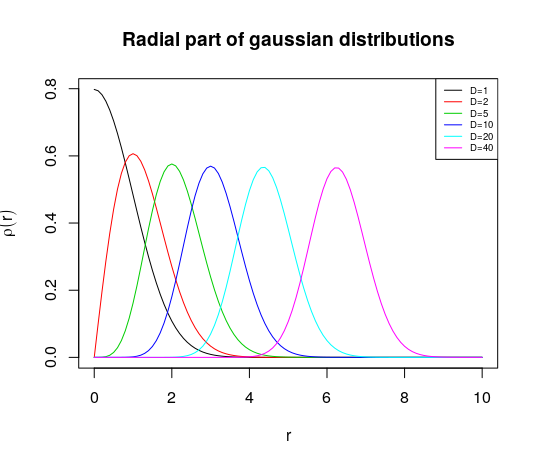
\includegraphics{c1f1}
\end{figure}

It was generated using the following R code.
\begin{lstlisting}[language=R, frame=single]
# Surface area of a unit hypersphere of D dimensions.
surface_area <- function(D) {
  2 * pi^(D/2)/gamma(D/2)
}

rho <- function(D, r) {
  surface_area(D) * r^(D - 1) * exp(-r^2/2)/(2 * pi)^(D/2)
}

r.vals <- seq(from = 0, to = 10, by = 0.1)

plot(
  r.vals,
  rho(1, r.vals),
  type = "l",
  col = 1,
  xlab = expression(r),
  ylab = expression(rho(r)),
  main = "Radial part of gaussian distributions"
)

plot_p <- function(D, n) {
  lines(r.vals, rho(D, r.vals), col = n)
}

sample_set <- data.frame(dim = c(2, 5, 10, 20, 40),
                         col = c(2, 3, 4, 5, 6))
apply(sample_set, 1, function(x)
  plot_p(x[1], x[2]))
legend(
  "topright",
  legend = paste(sep = "", "D=", c(1, sample_set$dim)),
  col = c(1, sample_set$col),
  lty = rep(1, 6),
  cex = 0.6
)

\end{lstlisting}

\item If $a \le b$, $a^2 \le ab$ and hence $a \le \sqrt{ab}$. Consider equation (1.78) of the book.
Its first term is 
\[
T_1 = \int_{\mathcal{R}_1}p(x, C_2)dx \le \int_{\mathcal{R}_1}\sqrt{p(x, C_1)p(x, C_2)}dx.
\]
This is because if the decision boundaries are correctly set, $p(x, C_2) \le p(x, C_1)$ in the region
$\mathcal{R}_1$. Similarly, the second term is
\[
T_2 = \int_{\mathcal{R}_2}p(x, C_1)dx \le \int_{\mathcal{R}_2}\sqrt{p(x, C_1)p(x, C_2)}dx.
\]
The probability of making a mistake is
\[
T_1 + T_2 \le \int_{\mathcal{R}}\left(p(x, C_1)p(x, C_2)\right)^{1/2}dx,
\]
where the region $\mathcal{R}$ is a union of regions $\mathcal{R}_1$ and $\mathcal{R}_2$.

\item The matrix $((L_{ij}))$ has all ones except the main diagonal which has all zeros. A
new $x$ is assigned to class $j$ for which the quantity
\[
\sum_{k}L_{kj}p(C_k|x) = \sum_k (1 - \delta_{kj})p(C_k|x) = \sum_k p(C_k|x) - p(C_j|x) = 1 - p(C_j|x)
\]
is minimal. Therefore, we end up selecting the class for which the posterior probability
is maximal.

\item We cannot classify unless we have the posterior probability $p(C_k|x)$. According to equation
(1.81), we choose that $j$ for which the quantity $\sum_k L_{kj}p(C_k|x)$ is minimal. The 
criterion can be written as
\[
i = \argmin_{1 \le j \le K}\left\{\sum_k L_{kj}p(C_k|x)\right\},
\]
where $K$ is the total number of classes.

\item The problem states that the loss incurred in the reject option is $\lambda$. In other
words, if the expected loss exceed $\lambda$ then we do not classify. Thus, we select class 
$C_i$ if
\[
i = \argmin_{1 \le j \le K}\left\{\sum_k L_{kj}p(C_k|x)\right\},
\]
and if 
\[
\sum_{k} L_{ki}p(C_k|x) < \lambda.
\]
If $L_{ki} = 1 - \delta_{ki}$ then the previous inequality is
\[
1 - \sum_{k}\delta_{ki}p(C_k|x) = 1 - p(C_i|x) < \lambda 
\]
which is equivalent to $p(C_i|x) > 1 - \lambda$. Recall, that this is the criterion for 
selection \emph{without} invoking the reject option. The reject option is invoked when
$p(C_i|x) \le 1 - \lambda$. Thus $\theta$ mentioned in section 1.5.3 is the same as $1 - \lambda$.

\item The expectation value of the loss is
\[
\ev(L(t, y(x))) = \iint \norm{y(x) - t}^2p(x, t)dxdt,
\]
where $x \in \sor^n$, $t \in \sor^m$ and $y:\sor^n \to \sor^m$. We can write $\norm{y(x) - t}^2 =
(y^T(x) - t^T)(y(x) - t)$ so that the functional derivative of this equation with respect to $y(x)$ is
\[
\frac{\delta}{\delta y(x)}\norm{y(x) - t}^2 = 2(y(x) - t).
\]
Then
\[
\frac{\delta\ev(L(t, y(x)))}{\delta x} = 2\int (y(x) - t)p(x,t)dt.
\]
At an extremum,
\[
\int (y(x) - t)p(x, t)dt = 0,
\]
or $y(x) = \int t p(x, t)dt = \ev_t(t|x)$.

\item We write the norm $N = \norm{y(x) - t}^2$ as 
\begin{eqnarray*}
N &=& \norm{y(x) - \ev_t(t|x) + \ev_t(t|x) - t}^2 \\
 &=& \norm{y(x) - \ev_t(t|x)}^2 + \norm{\ev_t(t|x) - t}^2 + \\
 & & (y(x) - \ev_t(t|x))^T(\ev(t|x) - t) + (\ev(t|x) - t)^T(y(x) - \ev_t(t|x)).
\end{eqnarray*}

The third term, after multiplying with $p(x,t)$ and integrated with respect to $t$ is
\[
\int (y(x) - \ev_t(t|x))^T(\ev(t|x) - t)p(x, t)dt = (y(x) - \ev_t(t|x))\left(\ev_t(t|x)\cdot 1 - \int t p(x,t)dt\right) 
\]
The second factor on the right hand side is zero because of which the integral vanishes. Note
that $\ev_t(x|t)$ is a function of $x$.

The fourth term is just the transpose of the third term and therefore vanishes. Therefore,
\[
\ev(L(t, y(x))) = \iint\norm{y(x) - \ev_t(t|x)}^2dxdt + \iint\norm{\ev_t(t|x) - t}^2dxdt.
\]
The only way to minimize the left hand side over the function $y$ is to let it be equal to $\ev_t(t|x)$.
This leaves the irreducible loss as
\[
\ev(L(t, y(x))) = \iint\norm{\ev_t(t|x) - t}^2dxdt.
\]

\item From equation (1.91),
\[
\ev(L_1) = \iint |y(x) - t|p(x, t)dxdt = \int_{\sor^n}\int_{\sor}|y(x) - t|p(x,t)dxdt,
\]
where we have assumed that $x \in \sor^n, t \in \sor$ and $y: \sor^n \to \sor$. We can split
the integral over $t$ to ensure that the integrand is always positive. Thus,
\[
\ev(L_1) = \int_{\sor^n}\int_{-\infty}^{y(x)} (y(x) - t)p(x, t)dxdt + \int_{\sor^n}\int_{y(x)}^{\infty}(t - y(x))p(x, t)dxdt.
\]
We now take the functional derivative with respect to $y(x)$ to get
\[
\frac{\delta\ev(L_1)}{\delta y(x)} = \int_{-\infty}^{y(x)}p(x,t)dt - \int_{y(x)}^{\infty}p(x, t)dt.
\]
At the extremum, the left hand side vanishes so that
\[
\int_{-\infty}^{y(x)}p(x,t)dt = \int_{y(x)}^{\infty}p(x, t)dt.
\]
Thus, $y(x)$ is the conditional median of $t$ given an $x$.

I do not know of even a passably rigorous argument to conclude that $y(x)$ is the conditional 
mode in the case $q \to 0$.

\item There is another way to infer that $h(p) \propto \ln p$. We use a slightly different notation
from the one used in the text. The relation between the densities is $p(x, y) = p_X(x)p_Y(y)$ and
that between information is $h(p) = h(p_X) + h(p_Y)$. Therefore, $a^{h(p)} = a^{h(p_X)}a^{h(p_Y)}$,
for any real constant $a$. Thus, $a^{h(p)} \propto p$ or $h(p) \propto ln p$, where the constant 
$\ln a$ is absorbed into the constant of proportionality.

We can arrive at the same conclusion by taking logarithm of $p(x,y) = p_X(x)p_Y(y)$.

\item The entropy of a discrete random variable is
\[
H(X) = -\sum_{i=1}^Mp(x_i)\log_2 p(x_i) = \sum_{i=1}^M p(x_i)\log_2\left(\frac{1}{p(x_i)}\right)
\]
Jensen's inequality for concave functions is
\[
f\left(\sum_{i=1}^M \lambda_i x_i\right) \ge \sum_{i=1}^M \lambda_i f(x_i).
\]
Choose $\lambda_i = p_i$, $x_i = 1/p_i$ and $f = \log_2$ so that
\[
\log_2\left(\sum_{i=1}^M p(x_i)\frac{1}{p(x_i)}\right) \ge \sum_{i=1}^M p(x_i)\log_2\left(\frac{1}{p(x_i)}\right).
\]
or $\log_2 M \ge H(X)$. 

Note that $\ln M = \ln 2 \log_2 M$ so that $\ln M < \log_2 M$. Therefore, we cannot conclude
that $\ln M \ge H(X)$.

\item The Kullback-Leibler divergence between distributions $p$ and $q$ is
\[
\kl(p || q) = -\int p(x)\ln\left(\frac{q(x)}{p(x)}\right)dx.
\]
If $p(x) = \mathcal{N}(x|\mu,\sigma)$ and $q(x) = \mathcal{N}(x|m, s)$ then
\begin{eqnarray*}
p(x) &=& \frac{1}{\sqrt{2\pi\sigma^2}}\exp\left(-\frac{(x - \mu)^2}{\sigma^2}\right) \\
q(x) &=& \frac{1}{\sqrt{2\pi s^2}}\exp\left(-\frac{(x - m)^2}{s^2}\right)
\end{eqnarray*}
so that
\[
\frac{q(x)}{p(x)} = \frac{\sigma}{s}\exp\left(\frac{(x - \mu)^2}{\sigma^2} - \frac{(x - m)^2}{s^2}\right)
\]
and hence
\[
\ln\left(\frac{q(x)}{p(x)}\right) = \ln\left(\frac{\sigma}{s}\right) + \frac{(x - \mu)^2}{\sigma^2} - \frac{(x - m)^2}{s^2}
\]
$\kl(p||q)$ is thus the sum of three integrals $I_1, I_2, I_3$, where
\begin{eqnarray*}
I_1 &=& -\ln\left(\frac{\sigma}{s}\right)\int_\sor p(x) dx = -\ln\left(\frac{\sigma}{s}\right) \\
I_2 &=& -\int_\sor \frac{(x - \mu)^2}{\sigma^2} p(x)dx \\
I_3 &=& \int_\sor \frac{(x - m)^2}{s^2}p(x)dx
\end{eqnarray*}
Consider $I_2$. Let $u = (x - \mu)/\sigma$ so that 
\[
I_2 = -\sigma\int_\sor \frac{u^2}{\sigma\sqrt{2\pi}}e^{-u^2/2}du = -\frac{1}{\sqrt{2\pi}}\int_{\sor} u^2 e^{-u^2/2}du.
\]
Using equation \eqref{c1pe9}, we get $I_2 = -1$.
Now consider
\[
I_3 = \int_\sor\frac{(x - m)^2}{s^2}p(x)dx = \int_\sor\frac{(x - \mu + \mu - m)^2}{\sigma^2}\frac{\sigma^2}{s^2}p(x)dx,
\]
or
\begin{eqnarray*}
I_3 &=& \frac{\sigma^2}{s^2}\int_\sor\frac{(x - \mu)^2}{\sigma^2}p(x)dx + \frac{2(\mu - m)}{s^2}\int_\sor (x-\mu)p(x)dx + \\
 & &  \frac{(\mu - m)^2}{s^2}\int_\sor p(x)dx
\end{eqnarray*}
Of these, the first integral is just $-I_2 = 1$. The second integral vanishes because the integrand
is an odd function around $\mu$ and the limits are symmetric around it. The third integral is $1$ 
following the normalization property of $p$. Therefore,
\[
I_3 = \frac{\sigma^2}{s^2}\left(1 + \frac{(\mu - m)^2}{\sigma^2}\right)
\]
and hence
\[
\kl(p || q) = -\ln\left(\frac{\sigma}{s}\right) - 1 + \frac{\sigma^2}{s^2} + \frac{(\mu - m)^2}{s^2}.
\]
It is easily verified that if $\mu = m$ and $\sigma = s$ then $\kl(p || q)$ vanishes.

\item The mutual information between two random variables, $X$ and $Y$ is
\[
I(X, Y) = H(Y) - H(Y|X).
\]
It is a non-negative quantity so that $H(Y) \ge H(Y|X)$. We also have $H(X, Y) = H(X) + H(Y|X)$
so that $H(Y) \ge H(X, Y) - H(X)$ or $H(X, Y) \le H(X) + H(Y)$. If $X$ and $Y$ are statistically
independent then $I(X, Y) = 0$ from which it immediately follows that $H(X, Y) = H(X) + H(Y)$.

\item We will first argue that if $Y = AX$, where $X, Y \in \sor^n$ are random vectors and $A$ is
a non-singular matrix then $p_Y(y) = \abs{\det{A}}^{-1}p_X(x)$. The probability of $X$ taking a value
in a neighbourhood $dx$ around $x$ is $p_X(x)dx$. This is the same as the probability of $AY$ taking
a value in a neighbourhood $d(Ay) = \abs{\det{A}}dy$ around $y$. Therefore, $p_X(x) = \abs{\det{A}}p_Y(y)$ 
or $p_Y(y) = \abs{\det{A}}^{-1}p_X(x)$.

Since $y = Ax$, we also have $dy = \abs{\det{A}}dx$. Therefore,
\begin{eqnarray*}
H(Y) &=& -\int p_Y(y)\ln p_Y(y)dy \\
     &=& -\int \abs{\det{A}}^{-1}p_X(x)\left(\ln\abs{\det{A}}^{-1} + \ln p_X(x)\right)\abs{\det{A}}dx \\
     &=& -\ln\abs{\det{A}}^{-1}\int p_X(x)dx - \int p_X(x)\ln p_X(x)dx \\
     &=& \ln\abs{\det{A}} + H(X).
\end{eqnarray*}

\item The conditional entropy $H(Y|X)$ between two discrete random variables $X$ and $Y$ is
\[
H(Y|X) = \sum_{x, y} p(x, y)\log\left(\frac{p(x, y)}{p(x)}\right).
\]
It is zero if and only if $p(x, y) = p(x)$ or that $p(y|x) = 1$. The latter is true if and only if
$Y$ is a function of $X$.

\item Consider the functional
\[
\begin{split}
f[p] =& -\int_\sor p(x)\ln p(x)dx - \lambda_1\left(\int_\sor p(x)dx - 1\right) \\
      & -\lambda_2\left(\int_\sor xp(x)dx - \mu\right) - \lambda_3\left(\int_\sor (x - \mu)^2p(x)dx - \sigma^2\right)
\end{split}
\]
Note that we have flipped the signs of the multipliers to ensure that the form of $p$ allows 
us to integrate it over $\sor$. The functional derivative of $f$ with respect to $p$ involves 
the following results,
\begin{eqnarray*}
I[p] = \int_\sor f(x)p(x)dx &\Rightarrow& \frac{\delta I}{\delta p} = f(x) \\
J[p] = \int_\sor p(x)\ln p(x)dx &\Rightarrow& \frac{\delta J}{\delta p} = 1 + \ln p(x).
\end{eqnarray*}
We will prove them after solving this problem. Thus,
\[
\frac{\delta f}{\delta p} = -1 - \ln p(x) - \lambda_1 - \lambda_2 x - \lambda_3 (x - \mu)^2.
\]
The functional derivative is zero when $\ln p(x) = -1 - \lambda_1 - \lambda_1 x - \lambda_3(x - \mu)^2$ 
or when
\[
p(x) = \exp\left(-1 - \lambda_1 - \lambda_2 - \lambda_2 (x - \mu)^2\right).
\]

We will now prove the two functional derivative results. Consider 
\[
I[p + \epsilon\eta(x)] = \int_\sor p(x)f(x)dx + \epsilon\int_\sor \eta(x)f(x)dx = I[p] + \epsilon\int_\sor\eta(x)f(x)dx
\]
so that
\[
\frac{\delta I}{\delta p} = f(x).
\]

Now consider
\[
J[p(x) + \epsilon\eta(x)] = \int_\sor p(x)\ln p(x)dx + \epsilon\int_\sor\eta(x)(1 + \ln p(x))dx,
\]
where we have ignored terms of second and higher orders in $\epsilon$. Therefore,
\[
\frac{\delta J}{\delta p} = 1 + \ln p(x).
\]

We now substitute (1.108) into the constraint equation (1.105), (1.106) and (1.107) to get
values of the three unknown Lagrange multipliers. The normalization constraint implies that
\begin{equation}\label{c1pe20}
\int_\sor e^{-\lambda_2 x - \lambda_3(x - \mu)^2}dx = e^{1 + \lambda_1}.
\end{equation}
The integral on the left hand side is evaluated after two changes in variable. Let $u = x - \mu$.
Then the integral, let us call it $I_1$ becomes
\[
I_1 = e^{-\lambda_2\mu}\int_\sor e^{-\lambda_2 u - \lambda_3 u^2}du
\]
We can write the integrand as
\[
\exp\left(-\lambda_3 u^2 - \lambda_2 u\right) = \exp\left[-\left(u\sqrt{\lambda_3} + \frac{\lambda_2}{2\sqrt{\lambda_3}}\right)^2 + \frac{\lambda_2^2}{4\lambda_3}\right]
\]
so that
\[
I_1 = \exp\left(-\lambda_2\mu + \frac{\lambda_2^2}{4\lambda_3}\right)\int_\sor\exp\left[-\left(u\sqrt{\lambda_3} + \frac{\lambda_2}{2\sqrt{\lambda_3}}\right)^2\right]du.
\]
We next introduce the variable
\[
v = u\sqrt{\lambda_3} + \frac{\lambda_2}{2\sqrt{\lambda_3}}
\]
so that
\[
I_1 = \exp\left(-\lambda_2\mu + \frac{\lambda_2^2}{4\lambda_3}\right)\frac{1}{\sqrt{\lambda_3}}\int_\sor e^{-v^2}dv
\]
or
\begin{equation}\label{c1pe21}
I_1 = \exp\left(-\lambda_2\mu + \frac{\lambda_2^2}{4\lambda_3}\right)\sqrt{\frac{\pi}{\lambda_3}}.
\end{equation}
From equations \eqref{c1pe20} and \eqref{c1pe21} we get
\begin{equation}\label{c1pe22}
1 + \lambda_1 + \lambda_2\mu - \frac{\lambda_2^2}{4\lambda_3} = \ln\sqrt{\frac{\pi}{\lambda_3}}.
\end{equation}

The constraint of equation (1.107) gives
\[
\int_\sor (x - \mu)^2e^{-\lambda_2 x - \lambda_3(x - \mu)^2}dx = \sigma^2 e^{1 + \lambda_1}.
\]
Let us denote by $I_3$ the integral on the left hand side. By using the same changes in variables
as before we get
\begin{equation}\label{c1pe23}
\exp\left(-\lambda_2\mu + \frac{\lambda_2^2}{4\lambda_3}\right)\frac{\sqrt{\pi}}{2\lambda_3^{3/2}}\left(1 + \frac{\lambda_2^2}{4\lambda_3}\right) = \sigma^2 e^{1 + \lambda_1}.
\end{equation}
We arbitrarily select $\lambda_2 = 0$ so that equations \eqref{c1pe22} and \eqref{c1pe23} become
\begin{eqnarray*}
1 + \lambda_1 &=& \ln\sqrt{\frac{\pi}{\lambda_3}} \\
\frac{\sqrt{\pi}}{2\lambda_3^{3/2}} &=& \sigma^2 e^{1 + \lambda_1}
\end{eqnarray*}
We can readily solve these equations to get $\lambda_1 = \ln\sqrt{2\pi\sigma^2} - 1$ and 
$\lambda_3 = (2\sigma^2)^{-1}$. The density $p$ is then
\[
p(x) = \frac{1}{\sqrt{2\pi\sigma^2}}\exp\left(-\frac{(x - \mu)^2}{2\sigma^2}\right).
\]

\item If $p$ is a univariate normal distribution,
\[
\ln p = \ln\left(\frac{1}{\sqrt{2\pi\sigma^2}}\right) - \frac{(x - \mu)^2}{2\sigma^2}
\]
and hence
\[
H = -\ln\left(\frac{1}{\sqrt{2\pi\sigma^2}}\right)\int_\sor p(x)dx + \frac{1}{2\sigma^2}\int_\sor (x - \mu)^2 p(x)dx.
\]
Using the constraints of equations (1.105) and (1.107) we get
\[
H = \frac{1}{2}\ln(2\pi\sigma^2) + \frac{1}{2} = \frac{1}{2}[1 + \ln(2\pi\sigma^2)].
\]

\item We first develop a convenient definition of the second derivative.
\begin{eqnarray*}
f^\prime(x) &=& \lim_{k \to 0}\frac{f(x+k) - f(x)}{k} \\
f^\prime(x+h) &=& \lim_{k \to 0}\frac{f(x+h+k) - f(x+h)}{k}
\end{eqnarray*}
Then,
\[
f^{\prime\prime}(x) = \lim_{h \to 0}\frac{f^\prime(x+h) - f^\prime(x)}{h} = \lim_{h,k \to 0}\frac{f(x+h+k) - f(x+h) - f(x+k) + f(x)}{hk}.
\]
Now choose $k = -h$ so that
\begin{equation}\label{c1pe24}
f^{\prime\prime}(x) = \lim_{h \to 0}\frac{f(x+h) + f(x-h) - 2f(x)}{h^2}.
\end{equation}
As 
\[
x = \frac{1}{2}(x + h) + \frac{1}{2}(x - h),
\]
the convexity of $f$ implies that
\[
f(x) \le \frac{1}{2}f(x+h) + \frac{1}{2}f(x-h)
\]
Using this in equation \eqref{c1pe23} proves that $f^{\prime\prime}(x) \ge 0$.

\item We start with
\[
H(X, Y) = \iint p(x, y)\ln p(x, y)dxdy.
\]
Since $p(x, y) = p(y|x)p(x)$,
\begin{eqnarray*}
H(X, Y) &=& \iint p(x, y)\ln p(y|x)dxdy + \iint p(x, y)\ln p(x)dxdy \\
 &=& H(Y|X) + \int\left(\int p(x, y)dy\right)\ln p(x)dx \\
 &=& H(Y|X) + H(X).
\end{eqnarray*}

\item We can write left hand side of (1.115) as
\[
f\left(\lambda_1 x_1 + \sum_{i=2}^{M-1}\lambda_i x_i\right).
\]
But induction hypothesis we can conclude that
\[
f\left(\lambda_1 x_1 + \sum_{i=2}^{M-1}\lambda_i x_i\right) \le f(\lambda_1 x_1) + f\left(\sum_{i=2}^{M} \lambda_i x_i\right).
\]
We can use the induction hypothesis once again on the second term to get the desired result.

\item 
\begin{enumerate}
\item $H(X) = -\frac{2}{3}\ln\frac{2}{3} - \frac{1}{3}\ln\frac{1}{3}$.
\item $H(Y) = -\frac{1}{3}\ln\frac{1}{3} - \frac{2}{3}\ln\frac{2}{3}$.
\item $H(Y|X) = -\sum_{x,y} p(x, y)\ln p(y|x) = -\frac{1}{3}\ln\frac{1}{2} - \frac{1}{3}\ln\frac{1}{2} - 0 - \frac{1}{3}\ln 1$.
\item $H(X|Y) = -\sum_{x,y} p(x, y)\ln p(x|y) = -\frac{1}{3}\ln 1 - 0 - \frac{1}{3}\ln\frac{1}{2} - \frac{1}{3}\ln\frac{1}{2}$.
\item $H(X, Y) = -\ln\frac{1}{3}$.
\item The definition of mutual information is
\[
I(X, Y) = -\sum_{x,y}p(x, y)\ln\frac{p(x)p(y)}{p(x, y)}.
\]
Therefore,
\[
I(X, Y) = -\frac{1}{3}\ln\frac{\frac{2}{3}\frac{1}{3}}{\frac{1}{3}} - \frac{1}{3}\ln\frac{\frac{2}{3}\frac{2}{3}}{\frac{1}{3}} - \frac{1}{3}\ln\frac{\frac{1}{3}\frac{2}{3}}{\frac{1}{3}}.
\]
\end{enumerate}

\item Since $\log$ is a concave function,
\[
\log\left(\frac{x_1}{2} + \frac{x_2}{2}\right) \ge \frac{1}{2}\log x_1 + \frac{1}{2}\log x_2 = \log\sqrt{x_1x_2}.
\]

\item Since $p(x, y) = p(y|x)p(x)$,
\begin{eqnarray*}
I(X, Y) &=& -\iint p(x, y)\ln\left(\frac{p(y)}{p(y|x)}\right)dxdy \\
 &=& -\iint p(x, y)\ln p(y) dxdy - \iint p(x, y)\ln p(y|x)dxdy.
\end{eqnarray*}
The first term on extreme right can be written as
\[
-\int\left(\int p(x, y)dx\right)\ln p(y)dy = -\int p(y)\ln p(y)dy = H(Y).
\]

\end{enumerate}


\chapter{Probability Distributions}\label{c2}
\section{Multinomial variables}\label{c2s1}
A multinomial variable can take one out of $K$ possible values. One can express it as a variable
with a range restricted to $K$ integers, typically $1$ to $K$. Alternatively, we can express it as 
a boolean  $K$ vector where exactly one component is $1$ and the rest are $0$. We choose the latter 
alternative. We use the notation customary in linear algebra to denote the boolean vector with just 
the $k$-th component $1$ and the remaining ones zero by $e_k$.

Let a multinomial variable $X$ take a value $k$ with probability $\mu_k$. Then 
\[
\sum_{k=1}^K \mu_k = 1
\]
and 
\begin{equation}\label{c2s1e1}
p(X = e_k|\mu) = \prod_{k=1}^K \mu_k^{x_k},
\end{equation}
where $x_k$ is the $k$th component of the boolean $K$-vector representing the state
$X = k$. Every component of the vector contributes a $1$ to the product except the
one with $x_k = 1$, which contributes $\mu_k$. Therefore,
\[
p(X = e_k|\mu) = \mu_k
\]
and hence
\begin{equation}\label{c2s1e2}
\sum_{k=1}^K`p(X = e_k|\mu) = 1.
\end{equation}

The expectation of a multinomial random variable is
\begin{equation}\label{c2s1e3}
\ev(X|\mu) = \sum_{k=1}^K e_kp(X = e_k|\mu) = (\mu_1, \ldots, \mu_K) = \mu.
\end{equation}
A dataset $\mathcal{D}$ of $N$ i.i.d. multinomial random variables has a prior probability
\[
p(\mathcal{D}|\mu) = \prod_{n=1}^Np(X_n = e_k|\mu) = \prod_{n=1}^N\prod_{k=1}^K \mu_k^{(x_n)_k}.
\]
In this equation, the data set has vectors ${x_1, \ldots, x_N}$, all in $\{0, 1\}^K$ and whose
$k$-th component is denoted by $(x_n)_k$. We can simplify the previous equation as
\[
p(\mathcal{D}|\mu) = \prod_{k=1}^K \mu_k^{\sum_{n=1}^N (x_n)_k}.
\]
The sum 
\[
\sum_{n=1}^N (x_n)_k
\]
is the number of $x_n$ whose $k$th component is $1$, that is the number of $x_n = e_k$. Let
us call this number $m_k$, Then
\begin{equation}\label{c2s1e4}
p(\mathcal{D}|\mu) = \prod_{k=1}^K \mu_k^{m_k}.
\end{equation}
It is clear that 
\begin{equation}\label{c2s1e5}
\sum_{k=1}^K m_k = N.
\end{equation}

We could have arrived at equation \eqref{c2s1e4} with a much simpler analysis. If the probability
that a multinomial random variable takes a value $k$ is $\mu_k$ and if a data set of $N$ such
variables has $m_k$ variables taking the value $k$ then
\[
p(\mathcal{D}|\mu) = \prod_{k=1}^K \mu_k^{m_k}.
\]
We took the longer route only to demonstrate how to work with boolean $K$-vectors.

In order to find the maximum-likelihood estimate of the $\mu$, we maximize the logarithm of
equation \eqref{c2s1e4} subject to the constraint $\sum_{k=1}^K \mu_k = 1$. If $\lambda$ is
the Lagrange's undermined multiplier then we consider the function
\[
f(\mu_k) = \sum_{k=1}^Lm_k\ln{\mu_k} + \lambda\left(\sum_{k=1}^K \mu_k - 1\right)
\]
and its derivative
\[
\frac{df}{d\mu_k} = \frac{m_k}{\mu_k} + \lambda.
\]
The maximum likelihood estimate of $\mu$ is thus,
\begin{equation}\label{c2s1e6}
\mu_{ML} = -\frac{1}{\lambda}(m_1, \ldots, m_K).
\end{equation}
The multiplier $\lambda$ can be found by substituting the previous equation in the equation
of constraint. Thus,
\[
\sum_{k=1}^K \mu_k = -\sum_{k=1}^K \frac{m_k}{\lambda} = -\frac{1}{\lambda}\sum_{k=1}^K m_k = 1.
\]
From equation \eqref{c2s1e5} we have
\[
\lambda = -\frac{1}{N}.
\]
Therefore the maximum-likelihood estimate of \eqref{c2s1e6} becomes
\begin{equation}\label{c2s1e7}
\mu_{ML} = \left(\frac{m_1}{N}, \ldots, \frac{m_k}{N}\right).
\end{equation}

\section{Conditional gaussian distributions}\label{c2s2}
Let $x \in \sor^D$, $x_a \in \sor^M$, where $M < D$ and $x_b \in \sor^{D-M}$. Then we can consider 
the probability distribution over $x$ as a joint distribution over $x_a$ and $x_b$. Let us partition
the mean $\mu \in \sor^D$ and the covariance matrix $\Sigma$, a $D \times D$ matrix as
\begin{eqnarray}
\mu &=& \begin{pmatrix} \mu_a \\ \mu_b \end{pmatrix} \label{c2s2e1} \\
\Sigma &=& \begin{pmatrix} \Sigma_{aa} & \Sigma_{ab} \\ \Sigma_{ba} & \Sigma_{bb} \end{pmatrix} \label{c2s2e2}
\end{eqnarray}
The symmetry of $\Sigma$ guarantees that $\Sigma_{aa}$ and $\Sigma_{bb}$ are symmetric and 
$\Sigma_{ab} = \Sigma_{ba}^T$. Let the corresponding precision matrix be 
\begin{equation}\label{c2s2e3}
\Lambda = \Sigma^{-1} = \begin{pmatrix} \Lambda_{aa} & \Lambda_{ab} \\ \Lambda_{ba} & \Lambda_{bb} \end{pmatrix} 
\end{equation}
The precision matrix is also symmetric because of the symmetry of $\Sigma$. Therefore $\Lambda_{aa}$
and $\Lambda_{bb}$ are symmetric while $\Lambda_{ab} = \Lambda_{ba}^T$. 

We are interested in finding out $p(x_a|x_b)$. By definition, 
\[
p(x_a|x_b) = p(x_a, x_b)p(x_b),
\]
where $x_b$ takes a given value in $\sor^{D-M}$. One can always simplify the right hand side to get
the expression for $p(x_a|x_b)$. However, it is easier to first find out the mean and the variance
and then compute the normalization constant. We will demonstrate it here.

The argument of the exponent in the gaussian can be written as
\begin{eqnarray*}
-\frac{1}{2}(x-\mu)\Sigma^{-1}(x - \mu) &=& -\frac{1}{2}x^T\Sigma^{-1}x + \frac{1}{2}x^T\Sigma^{-1}\mu \\
 & & + \frac{1}{2}\mu^T\Sigma^{-1}x + \frac{1}{2}\mu^T\Sigma^{-1}\mu.
\end{eqnarray*}
Since $\Sigma^{-1}$ is a symmetric matrix,
\[
\mu^T\Sigma^{-1}x = \left(\mu^T\Sigma^{-1}x\right)^T = x^T\Sigma^{-1}\mu
\]
so that
\begin{eqnarray*}
-\frac{1}{2}(x-\mu)^T\Sigma^{-1}(x-\mu) &=& -\frac{1}{2}x^T\Sigma^{-1}x + x^T\Sigma^{-1}\mu - \\
 & & \frac{1}{2}\mu^T\Sigma^{-1}\mu
\end{eqnarray*}
Thus, the argument of the exponent is written as a sum of a term quadratic in $x$, linear in $x$
and a constant. Therefore, given any quadratic form, the term quadratic in $x$ gives the
covariance matrix. Knowing the covariance matrix, the linear term gives the mean.

In the case of $p(x_a|x_b)$, after expressing the argument of the exponent in $p(x_a, x_b)$ in
terms of the precision matrix, we get
\begin{equation}\label{c2s2e4}
\Sigma_{a|b} = \Lambda_{aa}^{-1}.
\end{equation}
The linear term in the exponent is $x^T(\Lambda_{aa}\mu_a - \Lambda_{ab}(x_b - \mu)b)$ so that
\begin{equation}\label{c2s2e5}
\mu_{a|b} = \Lambda_{aa}^{-1}(\Lambda_{aa}\mu_a - \Lambda_{ab}(x_b - \mu_b)) = \mu_a - \Lambda_{aa}^{-1}\Lambda_{ab}(x_b - \mu_b).
\end{equation}

\section{Problems}\label{c2p}
\begin{enumerate}
\item The Bernoulli distribution is defined as $\mathrm{Bern}(x|\mu) = \mu^x(1 - \mu)^x$. The 
random variable can take only two values, $0$ and $1$. Clearly, $p(X=0|\mu) = 1 - \mu$ and 
$p(X=1|\mu) = \mu$ so that
\[
\sum_x p(x|\mu) = 1.
\]
The expectation value of $X$ is
\[
\ev(X) = \sum_x xp(x|\mu) = 0\cdot(1 - \mu) + 1\cdot\mu = \mu.
\]
The variance of $X$ is
\[
\var(X) = \sum_x \ev(x - \mu)^2 = (0 - \mu)^2(1 - \mu) + (1 - \mu)^2\mu = \mu(1 - \mu).
\]

\item Given that
\[
p(x|\mu) = \left(\frac{1-\mu}{2}\right)^{(1-x)/2}\left(\frac{1+\mu}{2}\right)^{(1+x)/2},
\]
where $x \in {-1, 1}$ and $\mu \in [0, 1]$. Then $p(X=-1|\mu) = (1 - \mu)/2$ and $p(X=1|\mu)
= (1 + \mu)/2$ so that 
\[
\sum_x p(x|\mu) = 1.
\]
The expectation value of $X$ is
\[
\ev(X) = \sum_x xp(x|\mu) = -1\cdot\frac{1 - \mu}{2} + 1\cdot\frac{1 + \mu}{2} = \mu.
\]
We also find
\[
\ev(X^2) = \frac{1 - \mu}{2} + \frac{1 + \mu}{2} = 1
\]
so that $\var(X) = 1 - \mu^2$. We verify the variance using the other form,
\[
\var(X) = (-1 - \mu)^2\frac{1 - \mu}{2} + (1 - \mu)^2\frac{1 + \mu}{2} = 1 - \mu^2.
\]

\item We can show that the binomial distribution is normalized by evaluating the sum,
\[
\sum_{m=0}^N\binom{N}{m}\mu^m(1 - \mu)^{N-m} = (\mu + 1 - \mu)^N = 1.
\]
We used the binomial theorem to get the first equality.

\item Consider the expression,
\[
\sum_{k=0}^N \binom{N}{k}\mu^k(1 - \mu)^{N-k} = 0.
\]
Differentiate it with respect to $\mu$. Recall that $\mu \in [0, 1]$ so that the differentiation 
is well defined.
\[
\sum_{k=0}^N\binom{N}{k}k\mu^{k-1}(1 - \mu)^{N-k} - \sum_{k=0}^N\binom{N}{k}(N-k)\mu^k(1 - \mu)^{N-k-1} = 0.
\]
Multiply throughout by $\mu$ to get
\[
\sum_{k=0}^N\binom{N}{k}\mu^k(1 - \mu)^{N-k} = \mu N\sum_{k=0}^{N-1}\binom{N-1}{k}\mu^k(1 - \mu)^{N-k-1}.
\]
The left hand side is $\bar{X}$ while the right hand side is $\mu N$.

\item Consider the product
\[
\Gamma(a)\Gamma(b) = \int_0^\infty e^{-x}x^{a-1}dx\int_0^\infty e^{-y}y^{b-1}dy = \iint_{Q_1}e^{-x-y} x^{a-1}y^{b-1}dxdy,
\]
where $Q_1$ is the first quadrant. To evaluate this integral, introduce the variables $x = zt$
and $y = z(1 - t)$ or $z = x + y$ and $t = x/(x + y)$. The variable $z$ ranges from $0$ to 
$\infty$ while $t$ goes from $0$ to $1$. The jacobian of the transformation is
\[
\frac{\partial(x, y)}{\partial(z, t)} = \begin{vmatrix} x_z & x_t \\ y_z & y_t \end{vmatrix}
= \begin{vmatrix} t & z \\ 1 - t & -z \end{vmatrix} = -z.
\]
Therefore, 
\[
\Gamma(a)\Gamma(b) = \int_0^\infty\int_0^1 e^{z} z^{a-1}t^{a-1}z^{b-1}(-t)^{b-1}\abs*{\frac{\partial(x, y}{\partial(z, t)}}dzdt.
\]
The $z$ and the $t$ integrals factor out, so that
\[
\Gamma(a)\Gamma(b) = \int_0^\infty e^z z^{a+b-1}dz\int_0^1 t^{a-1}(1 - t)^{b- 1}dt = \Gamma(a+b)B(a, b).
\]

\item The mean of beta distribution is
\begin{eqnarray*}
\ev(X) &=& \frac{\Gamma(a+b)}{\Gamma(a)\Gamma(b)}\int_0^1 x B(x|a, b)dx \\
 &=& \frac{\Gamma(a+b)}{\Gamma(a)\Gamma(b)}\int_0^1x^a(1 - x)^{b-1}dx \\
 &=& \frac{\Gamma(a+b)}{\Gamma(a)\Gamma(b)}\frac{\Gamma(a+1)\Gamma(b)}{\Gamma(a+b+1)} \\
 &=& \frac{a}{a+b}.
\end{eqnarray*}
Likewise,
\begin{eqnarray*}
\ev(X^2) &=& \frac{\Gamma(a+b)}{\Gamma(a)\Gamma(b)}\int_0^1 x^2 B(x|a, b)dx \\
 &=& \frac{\Gamma(a+b)}{\Gamma(a)\Gamma(b)}\int_0^1x^{a+2}(1 - x)^{b-1}dx \\
 &=& \frac{\Gamma(a+b)}{\Gamma(a)\Gamma(b)}\frac{\Gamma(a+2)\Gamma(b)}{\Gamma(a+b+2)} \\
 &=& \frac{a(a+1)}{(a+b)(a+b+1)}.
\end{eqnarray*}
Therefore,
\[
\var{X} = \frac{a(a+1)}{(a+b)(a+b+1)} - \frac{a^2}{(a+b)^2} = \frac{ab}{(a+b)^2(a+b+1)}.
\]

The mode of the distribution is the maximum of $\mathrm{Beta}(X|a, b)$. Its derivative
with respect to $x$ is
\[
\frac{\Gamma(a+b)}{\Gamma(a)\Gamma(b)}\left((a-1)x^{a-2}(1-x)^{b-1} - (b-1)x^{a-1}(1-x)^{b-2}\right)
\]
The extremum is found by setting it equal to zero, which gives
\[
(a-1)(1 - x) = (b - 1)x
\]
or
\[
x = \frac{a-1}{a+b-2}.
\]

We can use the following R code to generate plots of beta distributions for various
values of $a$ and $b$.
\begin{lstlisting}[language=R, frame=single]
x <- seq(from = 0, to = 1, by = 0.01)
b.1 <- dbeta(x, 0.1, 0.1)
b.2 <- dbeta(x, 1, 1)
b.3 <- dbeta(x, 2, 3)
b.4 <- dbeta(x, 8, 4)
plot(x, 
     b.1, 
     type = "l", 
     xlab = "x", 
     ylab = "B(a, b)", 
     main = "Beta distributions")
lines(x, b.2, col = 2, lty = 2)
lines(x, b.3, col = 3, lty = 3)
lines(x, b.4, col = 4, lty = 4)
legend(locator(1), 
       legend = c("(0.1,0.1)","(1,1)","(2,3)","(8,4)"), 
       col = c(1,2,3,4), 
       lty = c(1,2,3,4), 
       cex = 0.7, 
       bty = "n")
\end{lstlisting}

\begin{figure}
\begin{center}
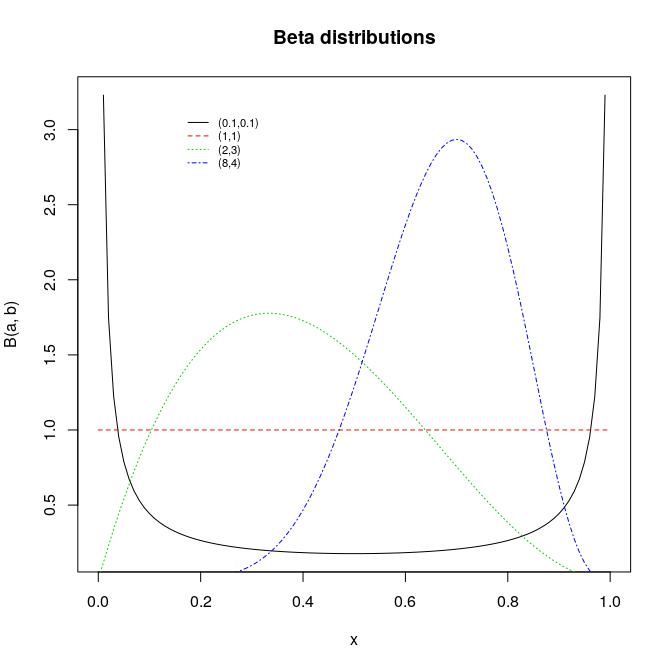
\includegraphics[scale=0.4]{c2f1}
\end{center}
\end{figure}

\item Let $X$ be a binomial random variable with probability mass function
\[
p(X = m|\mu) = \binom{N}{n}\mu^n (1 - \mu)^{N-n}.
\]
Let the parameter $\mu$ be described by a prior distribution
\begin{equation}\label{c2pe1}
\mathrm{Beta}(\mu|a, b) = \frac{\Gamma(a + b)}{\Gamma(a)\Gamma(b)}\mu^{a-1}(1 - \mu)^{b-1}.
\end{equation}
The observed data of $m + l$ realizations of $X$ has $x = 1$ $m$ times and $x = 0$ $l$ times.
Therefore, the likelihood function is
\[
p(\mathcal{D}|\mu) = \prod_{i=1}^{m}p(X=1|\mu)\prod_{j=1}^lp(X=0|\mu) = \mu^m(1 - \mu)^l.
\]
The posterior distribution of $\mu$ given the data $\mathcal{D}$ is
\[
p(\mu|D) \propto p(\mathcal{D}|\mu)\mathrm{Beta}(\mu|a, b) = \frac{\Gamma(a+b)}{\Gamma(a)\Gamma(b)}\mu^{m+a-1}(1-\mu)^{l+b-1}.
\]
The constant of proportionality is
\[
\frac{\Gamma(m+l+a+b)}{\Gamma(m+a)\Gamma(b+l)}
\]
so that
\[
p(\mu|\mathcal{D}) = \frac{\Gamma(m+l+a+b)}{\Gamma(m+a)\Gamma(b+l)}\mu^{m+a-1}(1-\mu)^{l+b-1}.
\]
The mean of $\mu$ conditioned on $\mathcal{D}$ is the posterior mean
\begin{equation}\label{c2pe2}
\mu_{post} = \frac{m+a}{m+a+l+b}.
\end{equation}

The log-likelihood function is
\[
\ln p(\mathcal{D}|\mu) = m\ln\mu + l\ln(1 - \mu)
\]
and its derivative is
\[
\frac{m}{\mu} - \frac{l}{1 - \mu}
\]
and its extremum is 
\begin{equation}\label{c2pe3}
\mu_{ML} = \frac{m}{m+l}.
\end{equation}
The mean of the prior distribution is that of equation \eqref{c2pe1}
\begin{equation}\label{c2pe4}
\mu_{prior} = \frac{a}{a+b}.
\end{equation}

Let us assume, for the moment that the maximum likelihood estimate is greater than the prior estimate.
That is,
\[
\mu_{ML} - \mu_{prior} > 0.
\]
This is possible if and only if 
\begin{equation}\label{c2pe5}
bm > al.
\end{equation}
If equation \eqref{c2pe5} is true then it is easy to verify that $\mu_{ML} > \mu_{post} > \mu_{prior}$. 
If \eqref{c2pe5} is not true then $\mu_{prior} \ge \mu_{post} \ge \mu_{ML}$.

\item Let $X$ and $Y$ be random variables with joint distribution $p(x, y)$. Then,
\[
\ev_x(X|Y) = \int xp(x|y)dx
\]
and 
\begin{eqnarray*}
\ev_y(\ev_x(X|Y)) &=& \int p(y)\ev_x(X|Y)dy \\
 &=& \iint xp(y)p(x|y)dxdy \\
 &=& \iint xp(x, y)dxdy \\
 &=& \ev(X).
\end{eqnarray*}

For sake of notational simplicity, let us denote $\ev_x(X|Y) = \phi(y)$. Then, 
\begin{equation}\label{c2pe6}
\var_y(\ev_x(X|Y)) = \var_y(\phi(y)) = \ev_y(\phi^2(y)) - (\ev_y\phi(y))^2
\end{equation}
Now, $\var_x(X|Y) = \ev_x(X^2|Y) - (\ev_x(X|Y))^2 = \ev_x(X^2|Y) - \phi^2(y)$ so that 
\[
\ev_y(\var_x(X|Y)) = \ev_y(\ev_x(X^2|Y)) - \ev_y(\phi^2(y))
\]
and hence
\[
\begin{split}
\var_y(\ev_x(X|Y)) + \ev_y(\var_x(X|Y)) =& \ev_y(\phi^2(y)) - (\ev_y\phi(y))^2 + \\
 & \ev_y(\ev_x(X^2|Y)) - \ev_y(\phi^2(y)) 
\end{split}
\]
and finally
\begin{equation}\label{c2pe7}
\var_y(\ev_x(X|Y)) + \ev_y(\var_x(X|Y)) = \ev_y(\ev_x(X^2|Y)) - (\ev_y\phi(y))^2 
\end{equation}
Now,
\begin{eqnarray*}
\ev_y(\ev_x(X^2|Y)) &=& \iint x^2 p(x|y)p(y)dxdy = \var(X) \\
\ev_y\phi(y) &=& \iint xp(x|y)p(y)dy = \ev(X)
\end{eqnarray*}
Using these in equation \eqref{c2pe7} we get the desired result.

\item We use the following result,
\begin{equation}\label{c2pe8}
\int_0^a x^{m-1}(a - x)^{n-1}dx = a^{m+n-1}B(m, n).
\end{equation}
To obtain it, we write the integral as
\[
a^{m+n-2}\int_0^a \left(\frac{x}{a}\right)^{m-1}\left(1 - \frac{x}{a}\right)^{n-1}ad\left(\frac{x}{a}\right).
\]
A transformation $x/a \mapsto y$ yields the result. The Dirichlet distribution is proportional
to 
\[
D = \prod_{k=1}^K\mu_k^{\alpha_k - 1}.
\]
subject to the constraint 
\begin{equation}\label{c2pe9}
\sum_{k=1}^K\mu_k = 1.
\end{equation}
Therefore, the distribution is proportional to
\[
D = \prod_{k=1}^{K-1}\mu_k^{\alpha_k - 1}(1 - \mu_1 - \cdots - \mu_{K-1})^{\alpha_K-1}
\]
The variables $\mu_k$ vary over $[0, 1]$. However, the constraint of equation \eqref{c2pe9} reduce the
region of integration from a hypercube to a $K-1$ simplex formed by the first quandrant and the plane whose 
equation is \eqref{c2pe9}. In order to find the normalization constant we must evaluate the integral
\begin{equation}\label{c2pe10}
I = \int_0^1\int_0^{1-\mu_1}\cdots\int_0^{1-\mu_1-\cdots-\mu_{K-2}}D(\mu_1, \ldots, \mu_{K-1})d\mu_1\cdots d\mu_{K-1}.
\end{equation}
The $\mu_{K-1}$ integral is
\begin{eqnarray*}
\int_0^{1-\mu_1-\cdots-\mu_{K-2}}\mu_{K-1}^{\alpha_K - 1}(1 - \mu_1 - \cdots - \mu_{K-1})^{\alpha_K-1}d\mu_{K-1} &=& \\
 (1-\mu_1-\cdots-\mu_{K-2})^{\alpha_K+\alpha_{K-1}-1}B(\alpha_K, \alpha_{K-1}) & &
\end{eqnarray*}
The integrals over the other variables are evaluated similarly so that
\[
I = B(\alpha_{K-1},\alpha_K)B(\alpha_{K-2},\alpha_{K}+\alpha_{K-1})\cdots B(\alpha_1,\alpha_{K}+\cdots+\alpha_2).
\]
Using the relation,
\[
B(m, n) = \frac{\Gamma(m)\Gamma(n)}{\Gamma(m+n)},
\]
we get
\begin{eqnarray*}
I &=& \frac{\Gamma(\alpha_{K-1})\Gamma(\alpha_K)}{\Gamma(\alpha_{K}+\alpha_{K-1})} \\
  & &  \frac{\Gamma(\alpha_{K-2})\Gamma(\alpha_K+\alpha_{K-1})}{\Gamma(\alpha_K+\alpha_{K-1}+\alpha_{K-2})}\cdots \\
  & &  \frac{\Gamma(\alpha_1)\Gamma(\alpha_K+\alpha_{K-1}+\cdots+\alpha_2)}{\Gamma(\alpha_K+\alpha_{K-1}+\cdots+\alpha_{1})}
\end{eqnarray*}
Cancelling common terms,
\[
I = \frac{\Gamma(\alpha_K)\Gamma(\alpha_{K-1})\cdots\Gamma(\alpha_1)}{\Gamma(\alpha_K+\alpha_{K-1}+\cdots+\alpha_1)}
\]
If we write $\alpha_0 = \alpha_1 + \cdots + \alpha_K$ then the normalization constant for the
Dirichlet distribution is
\[
\frac{\Gamma(\alpha_0)}{\Gamma(\alpha_1)\cdots\Gamma(\alpha_K)}.
\]

\item We start with the Dirichlet distribution
\[
\mathrm{Dir}(\mu|\alpha) = \frac{\Gamma(\alpha_0)}{\Gamma(\alpha_1)\cdots\Gamma(\alpha_K)}\prod_{k=1}^K\mu_k^{\alpha_k - 1},
\]
where $\mu, \alpha \in \sor^K$ and
\begin{eqnarray*}
\sum_{i=1}^K \mu_k &=& 1 \\
\sum_{i=1}^K \alpha_k &=& \alpha_0
\end{eqnarray*}
The mean of the distribution is
\begin{eqnarray*}
\ev(\mu_j) &=& \int\frac{\Gamma(\alpha_0)}{\Gamma(\alpha_1)\cdots\Gamma(\alpha_K)}\prod_{k=1}^K\mu_k^{\alpha_k + \delta_{jk} - 1}d\mu \\
 &=& \frac{\Gamma(\alpha_0)}{\Gamma(\alpha_1)\cdots\Gamma(\alpha_K)}\frac{\Gamma(\alpha_1)\cdots\Gamma(\alpha_j+1)\cdots\Gamma(\alpha_K)}{\Gamma(\alpha_0 + 1)} \\
 &=& \frac{\alpha_j}{\alpha_0}
\end{eqnarray*}
In order to find the variance, we need
\begin{eqnarray*}
\ev(\mu_j^2) &=& \int\frac{\Gamma(\alpha_0)}{\Gamma(\alpha_1)\cdots\Gamma(\alpha_K)}\prod_{k=1}^K\mu_k^{\alpha_k + 2\delta_{jk} - 1}d\mu \\
 &=& \frac{\Gamma(\alpha_0)}{\Gamma(\alpha_1)\cdots\Gamma(\alpha_K)}\frac{\Gamma(\alpha_1)\cdots\Gamma(\alpha_j+2)\cdots\Gamma(\alpha_K)}{\Gamma(\alpha_0 + 2)} \\
 &=& \frac{\alpha_j(\alpha_j+1)}{\alpha_0(\alpha_0+1)}
\end{eqnarray*}
Therefore,
\[
\var(\alpha_j) = \frac{\alpha_j(\alpha_j+1)}{\alpha_0(\alpha_0+1)} - \frac{\alpha_j^2}{\alpha_0^2} = \frac{\alpha_j(\alpha_0 - \alpha_j)}{\alpha_0^2(\alpha_0+1)}.
\]
Note that the definition of $\alpha_0$ guarantees us that the variance is non-negative. In order
to find the covariance, we need
\begin{eqnarray*}
\ev(\mu_i\mu_j) &=& \int\frac{\Gamma(\alpha_0)}{\Gamma(\alpha_1)\cdots\Gamma(\alpha_K)}\prod_{k=1}^K\mu_k^{\alpha_k + \delta_{ik} + \delta_{jk} - 1}d\mu \\
 &=& \frac{\Gamma(\alpha_0)}{\Gamma(\alpha_1)\cdots\Gamma(\alpha_K)}\frac{\Gamma(\alpha_1)\cdots\Gamma(\alpha_i+1)\cdots\Gamma(\alpha_j+1)\cdots\Gamma(\alpha_K)}{\Gamma(\alpha_0 + 2)} \\
 &=& \frac{\alpha_i\alpha_j}{\alpha_0(\alpha_0+1)}
\end{eqnarray*}
so that
\[
\cov(\mu_i\mu_j) = \frac{\alpha_i\alpha_j}{\alpha_0(\alpha_0+1)} - \frac{\alpha_i\alpha_j}{\alpha_0^2} = -\frac{\alpha_i\alpha_j}{\alpha_0^2(\alpha_0+1)}.
\]

\item Recall that the derivative of $a^x$ with respect to $x$ is $a^x\ln a$. Therefore,
\[
\frac{\partial}{\partial\alpha_j}\prod_{k=1}^K \mu_k^{\alpha_k-1} = \ln\mu_j\prod_{k=1}^K\mu_k^{\alpha_k-1}.
\]
Now,
\begin{eqnarray*}
\ev(\ln\mu_j) &=& \frac{\Gamma(\alpha_0)}{\Gamma(\alpha_1)\cdots\Gamma(\alpha_K)}\int\ln\mu_j\prod_{k=1}^K\mu_k^{\alpha_k-1}d\mu \\
 &=& \frac{\Gamma(\alpha_0)}{\Gamma(\alpha_1)\cdots\Gamma(\alpha_K)}\int\frac{\partial}{\partial\alpha_j}\prod_{k=1}^K\mu_k^{\alpha_k-1}d\mu \\
 &=& \frac{\Gamma(\alpha_0)}{\Gamma(\alpha_1)\cdots\Gamma(\alpha_K)}\frac{\partial}{\partial\alpha_j}\int\prod_{k=1}^K\mu_k^{\alpha_k-1}d\mu \\
 &=& \frac{\Gamma(\alpha_0)}{\Gamma(\alpha_1)\cdots\Gamma(\alpha_K)}\frac{\partial}{\partial\alpha_j}\frac{\Gamma(\alpha_1)\cdots\Gamma(\alpha_K)}{\Gamma(\alpha_0)} \\
 &=& \frac{\Gamma(\alpha_0)}{\Gamma(\alpha_j)}\frac{\partial}{\partial\alpha_j}\frac{\Gamma(\alpha_j)}{\Gamma(\alpha_0)} \\
 &=& \frac{1}{\Gamma(\alpha_j)}\frac{\partial}{\partial\alpha_j}\Gamma(\alpha_j) - \frac{1}{\Gamma(\alpha_0)}\frac{\partial}{\partial\alpha_j}\Gamma(\alpha_0) \\
 &=& \frac{\partial}{\partial\alpha_j}\ln\Gamma(\alpha_j) - \frac{\partial}{\partial\alpha_j}\ln\Gamma(\alpha_0) \\
 &=& \psi(\alpha_j) - \psi(\alpha_0),
\end{eqnarray*}
where 
\[
\psi(\alpha) = \frac{d}{d\alpha}\ln\Gamma(\alpha)
\]
is the digamma function.

\item The uniform distribution is defined by
\[
\mathrm{Unif}(x|a, b) = \frac{1}{b - a}, x \in [a, b].
\]
It is easy to confirm that it is normalized, for
\[
\int_a^b \mathrm{Unif}(x|a, b)dx = \frac{1}{b-a}\int_a^b dx = 1.
\]
The mean value of $x$ is
\[
\ev(x) = \int_a^b x\mathrm{Unif}(x|a, b)dx = \int_a^b \frac{x}{b-a}dx = \frac{1}{2(b-a)}(b^2 - a^2) = \frac{a+b}{2}.
\]
The mean value of $x^2$ is
\[
\ev(x^2) = \int_a^b\frac{x^2}{b-a}dx = \frac{1}{3(b-a)}(b^3-a^3) = \frac{a^2 + ab + b^2}{3}
\]
so that 
\[
\var(x) = \frac{a^2 + ab + b^2}{3} - \frac{(a+b)^2}{4} = \frac{(b - a)^2}{12}.
\]

\item Given that
\begin{eqnarray*}
p(x) &=& \mathcal{N}(x | \mu, \Sigma) \\
q(x) &=& \mathcal{N}(x | m, L),
\end{eqnarray*}
where $x, \mu, m \in \sor^n$ and $\Sigma, L$ are covariance matrices.
\[
\ln\left(\frac{q(x)}{p(x)}\right) = \frac{1}{2}\ln\frac{\det L}{\det\Sigma} - \frac{(x - m)^TL^{-1}(x - m)}{2} + \frac{(x - \mu)^T\Sigma^{-1}(x - \mu)}{2}.
\]
The Kullback-Leibler divergence between $p$ and $q$ is the sum of three integrals,
\begin{eqnarray*}
I_1 &=& -\frac{1}{2}\ln\left|\frac{\det L}{\det\Sigma}\right|\int_{\sor^n}p(x)dx \\
I_2 &=& \frac{1}{2}\int_{\sor^n}(x-m)^TL^{-1}(x-m)p(x)dx \\
I_3 &=& -\frac{1}{2}\int_{\sor^n}(x-\mu)^T\Sigma^{-1}(x-\mu)p(x)dx.
\end{eqnarray*}
It is easy to evaluate $I_1$ using normalization property of $p$.
\begin{equation}\label{c2pe11}
I_1 = -\frac{1}{2}\ln\left|\frac{\det L}{\det\Sigma}\right|.
\end{equation}
Using the definitions of expectations, we conclude that
\[
I_2 = \ev[(x - m)^TL^{-1}(x-m)].
\]
Using formula (380) of the matrix cookbook \cite{petersen2012matrix} we get
\begin{equation}\label{c2pe12}
I_2 = (m - \mu)^TL^{-1}(m - \mu) + \tr(L^{-1}\Sigma).
\end{equation}
In eaxctly the same manner, we conclude that
\begin{equation}\label{c2pe13}
I_3 = 0 + \tr(\Sigma^{-1}\Sigma) = n.
\end{equation}
Therefore,
\[
\kl(p||q) = -\frac{1}{2}\left(\ln\left|\frac{\det L}{\det\Sigma}\right| - (m - \mu)^T L^{-1}(m - \mu) + \tr(L^{-1}\Sigma) + d\right).
\]

\item Let $x, \mu \in \sor^n$ and $\Sigma$ be an $n \times n$ covariance matrix. The entropy of a 
distribution is given by
\[
H = -\int p(x)\ln p(x)dx.
\]
We want to maximize $H$ subject to the constraints
\begin{eqnarray}
\int p(x)dx &=& 1 \label{c2pe14} \\
\int xp(x)dx &=& \mu \label{c2pe15} \\
\int (x - \mu)(x - \mu)^Tp(x)dx &=& \Sigma \label{c2pe16} .
\end{eqnarray}
If $\lambda_1, \ell, \lambda_3$ are the Lagrange multipliers for each of these constraints then
we seek to maximize the functional
\begin{eqnarray*}
L[x] &=& H - \lambda_1\left(\int p(x)dx - 1\right) - \ell^T\left(\int xp(x)dx - \mu\right) - \\
 & & \Lambda\left(\int(x-\mu)^T(x-\mu)p(x)dx - \Sigma\right),
\end{eqnarray*}
where $\lambda_1 \in \sor, \ell \in \sor^n$ and $\Lambda$ is an $n \times n$ non-singular 
symmetric matrix. Each term on the right hand side is a number. Therefore, it is equal to the
trace of itself. We use this fact on the third term to get
\begin{eqnarray*}
L[x] &=& H - \lambda_1\left(\int p(x)dx - 1\right) - \ell^T\left(\int xp(x)dx - \mu\right) - \\
 & & \tr\left\{\Lambda\left(\int(x-\mu)^T(x-\mu)p(x)dx - \Sigma\right)\right\},
\end{eqnarray*}
 We now take the functional derivative of the above equation with respect to $p$,
\[
\frac{\delta L}{\delta p} = -1 - \ln p(x) - \lambda_1 - \ell^T x - \tr(\Lambda (x - \mu)^T(x - \mu)).
\]
As $\tr(AB) = \tr(BA)$, we can write the last expression on the right hand side as
\[
\frac{\delta L}{\delta p} = -1 - \ln p(x) - \lambda_1 - \ell^T x - \tr((x - \mu)^T\Lambda(x - \mu)).
\]
At an extremum of $L$, the functional derivative vanishes so that $\ln p(x) = -1 - \lambda_1 - \ell x
- (x - \mu)^T\Lambda(x - \mu)$ or
\begin{equation}\label{c2pe17}
p(x) = \exp\left(-1 - \lambda_1 - \ell^T x - (x - \mu)^T\Lambda(x - \mu)\right).
\end{equation}
We now write 
\begin{eqnarray*}
\ell^T x &=& \ell^T \Lambda^{-1} \Lambda x + \mu^T\ell - \mu^T\ell \\
 &=&  \ell^T \Lambda^{-1} \Lambda x + \mu^T\ell - \ell^T\mu \\
 &=& \ell^T\Lambda^{-1}\Lambda(x - \mu) + \mu^T\ell.
\end{eqnarray*}
We used the fact that $\mu^T\ell = (\mu, \ell) = (\ell, \mu) = \ell^T\mu$ as all
the vectors are real. Since $\Lambda$ is symmetric, so is its inverse and hence $\Lambda^{-1}
= (\Lambda^{-1})^T$. Therefore,
\begin{eqnarray*}
\ell^T x &=& (\ell\Lambda^{-1})^T\Lambda(x - \mu) + \mu^T\ell \\
 &=& \frac{(\ell\Lambda^{-1})^T\lambda_x(x - \mu)}{2} + \frac{(x - \mu)^T\Lambda^T\Lambda^{-1}\ell}{2} + \mu^T\ell
\end{eqnarray*}
and hence
\begin{eqnarray*}
\ell^Tx + (x-\mu)^T\Lambda(x-\mu) &=& \left(x-\mu+\frac{\Lambda^{-1}\ell}{2}\right)^T\Lambda\left(x-\mu+\frac{\Lambda^{-1}\ell}{2}\right) \\
 & & \mu^T\ell - \frac{\ell^T\Lambda^{-1}\ell}{4}
\end{eqnarray*}
The density $p$ can now be written as
\[
p(x)=\exp\left[-1-\lambda_1 - \left(x-\mu+\frac{\Lambda^{-1}\ell}{2}\right)^T\Lambda\left(x-\mu+\frac{\Lambda^{-1}\ell}{2}\right)-\mu^T\ell+\frac{\ell^T\Lambda^{-1}\ell}{4}\right]
\]
Introduce a variable 
\[
y = x - \mu + \frac{\Lambda^{-1}\ell}{2}
\]
so that the density becomes
\[
p(y) = \exp\left[-1-\lambda_1-y^T\Lambda y - \mu^T\ell - \frac{\ell^T\Lambda^{-1}\ell}{4}\right].
\]
We use this form in the second constraint to get
\[
\int\left(y + \mu + \frac{\Lambda^{-1}\ell}{2}\right)p(y)dy = \mu.
\]
The integral of $yp(y)$ vanishes because it is an odd function. The rest of the term evaluates to
\[
\mu + \frac{\Lambda^{-1}\ell}{2} = \mu
\]
or $\Lambda^{-1}\ell = 0$. As $\Lambda$ is a non-singular symmetric matrix, this means that $\ell = 0$.
The form of the density now simplifies to
\[
p(y) = \exp\left(-1 - \lambda_1 - y^T\Lambda y\right),
\]
where $y$ now is just $x - \mu$. We now use this form in the third constraint. We define 
$y = x - \mu$ so that
\begin{equation}\label{c2pe18}
\int yy^Te^{-1 - \lambda_1 - y^T\Lambda y}dy = \Sigma \Rightarrow e^{-1-\lambda_1} \int yy^T e^{-y^T\Lambda y}dy = \Sigma.
\end{equation}
In order to evaluate this integral we use the eigenvalues of $\Lambda$. Let $\Lambda u_i = \alpha_i u_i$,
where $u_i$ is an eigenvector corresponding to the eigenvalue $\alpha_i$. We can then write 
\[
y = \sum_{i=1}^n \beta_i u_i,
\]
where $\beta_i = u_i^T y = (u_i, y)$. The $n$ numbers $\beta_i$ form a vector $\beta$ and we can write
\begin{equation}\label{c2pe19}
\beta = Uy,
\end{equation}
where the matrix $U = [u_1 \ldots u_n]$ has the eigenvectors of $\Lambda$ as its columns. From \eqref{c2pe19}
we readily get 
\begin{equation}\label{c2pe20}
d\beta = \abs{\det U}dy.
\end{equation}
If we choose the eigenvectors to be orthonormal then $\abs{\det U} = 1$ and 
\begin{equation}\label{c2pe21}
d\beta = dy.
\end{equation}
Therefore,
\[
y^T\Lambda y = \sum_{i,j=1}^n \beta_i u_i^T \Lambda \beta_j u_j = \sum_{i,j=1}^n \beta_i\beta_j\alpha_j u_i^T u_j,
\]
where $\alpha_j$ is the eigenvalue of $u_j$. As the eigenvectors $\{u_i\}$ can always be 
assumed to be orthonormal, $(u_i, u_j) = \delta_{ij}$ and hence
\[
y^T\Lambda y = \sum_{i=1}^n \beta_j^2\alpha_i
\]
Recall that $\Lambda$ is a constant matrix. Therefore, its eigenvectors are also constant and hence
\[
y = \sum_{i=1}^n\beta_i u_i \Rightarrow dy = \sum_{i=1}^n u_i d\beta_i
\]
Equation \eqref{c2pe18} now becomes
\begin{equation}\label{c2pe22}
e^{-1+\lambda_1}\sum_{i,j=1}^nu_iu_j^T\int \exp\left(-\sum_{k=1}^n\beta_k^2\alpha_k\right)\beta_i\beta_j d\beta = \Sigma.
\end{equation}
The integral in the above equation is zero if $i \ne j$. When $i = j$, it becomes
\[
I = \int e^{-\beta_1^2\alpha_1}d\beta_1 \cdots \int \beta_i^2e^{-\beta_i^2\alpha_i}d\beta_i \cdots \int e^{-\beta_n^2\alpha_n}d\beta_n = \frac{\pi^{n/2}}{\sqrt{\alpha_1 \cdots \alpha_n}}\frac{1}{2\alpha_i}.
\]
Equation \eqref{c2pe22} then becomes
\[
e^{-1-\lambda_1}\sqrt{\frac{\pi^n}{\alpha_1\cdots\alpha_n}}\sum_{i=1}^n \frac{1}{2\alpha_i}u_iu_i^T = \Sigma.
\]
Since $\Lambda u_i = \alpha_i u_i$, the expression sum in the above equation is really $\Lambda^{-1}/2$.
(Refer to equations (2.48) and (2.49) of the book.). Therefore,
\[
e^{-1 - \lambda_1}\sqrt{\frac{\pi^n}{\alpha_1\cdots\alpha_n}}\frac{1}{2}\Lambda^{-1} = \Sigma.
\]
The determinant of a matrix is a product of its eigen-values. Therefore,
\[
\frac{e^{-1 - \lambda_1}}{2}\frac{\pi^{n/2}}{\sqrt{\det\Lambda}}\Lambda^{-1} = \Sigma.
\]
We now choose $\Lambda^{-1} = 2\Sigma$ so that
\begin{equation}\label{cpe23}
\Lambda = \frac{1}{2}\Sigma^{-1}.
\end{equation}
and $\lambda_1$ such that 
\[
e^{-1 - \lambda_1}\frac{\pi^{n/2}}{\sqrt{\det\Lambda}} = 1 \Rightarrow e^{-1-\lambda_1} = \frac{\sqrt{\det\Lambda}}{\pi^{n/2}}.
\]
From equation \eqref{cpe23}, 
\[
\det\Lambda = \frac{1}{2^n}\det\Sigma^{-1} = \frac{1}{2^n}\frac{1}{\det\Sigma}
\]
so that
\begin{equation}\label{cpe24}
e^{-1 - \lambda_1} = \frac{1}{(2\pi)^{n/2}}\frac{1}{\sqrt{\det\Sigma}}.
\end{equation}
Equations \eqref{cpe23}, \eqref{cpe24} and the fact that $\ell = 0$ make the $p$ a multi-variate
gaussian distribution.

\item The entropy of a distribution $p$ is
\[
H = -\int p(x)\ln p(x)dx.
\]
If $p$ is a multivariate gaussian distribution,
\[
p(x) = \frac{1}{(2\pi)^{n/2}}\frac{1}{\sqrt{\det\Sigma}}\exp\left(-\frac{(x - \mu)^T\Sigma^{-1}(x - \mu)}{2}\right)
\]
so that
\[
\ln p = -\frac{n}{2}\ln(2\pi) - \frac{1}{2}\ln\det\Sigma - \frac{(x - \mu)^T\Sigma^{-1}(x - \mu)}{2}
\]
Therefore,
\[
H = \frac{n}{2}\ln(2\pi) + \frac{1}{2}\ln\det\Sigma + \frac{1}{2}\int(x - \mu)^T\Sigma^{-1}(x - \mu)p(x)dx.
\]
The integral $I$ is best evaluated using the property of expectations. Clearly, $I = \ev((x-\mu)^T\Sigma^{-1}(x-\mu))$.
As $(x-\mu)^T\Sigma^{-1}(x-\mu)$ is a number, we can as well write
\begin{eqnarray*}
I &=& \ev(\tr((x - \mu)^T\Sigma^{-1}(x - \mu))) \\
  &=& \ev(\tr(\Sigma^{-1}(x - \mu)^T(x - \mu))) \\
  &=& \ev(\tr(\Sigma^{-1})\tr((x - \mu)^T(x - \mu))) \\
  &=& \tr(\Sigma^{-1})\ev(\tr((x - \mu)^T(x - \mu))) \\
  &=& \tr(\Sigma^{-1})\tr(\ev(x - \mu)^T(x - \mu)) \\
  &=& \tr(\Sigma^{-1})\tr(\Sigma) \\
  &=& \tr(\Sigma^{-1}\Sigma) = n
\end{eqnarray*}
The entropy is thus,
\[
H = \frac{1}{2}\ln\det\Sigma + \frac{n}{2}\left(1 + \ln(2\pi)\right).
\]

\item Given that the random variable $X$ is a sum of two gaussian random variables $X_1$ and $X_2$.
The probability that $X$ takes a value between $x$ and $x + dx$ is $p(x)dx$. This is equal to the
probability that $X_2$ takes a value between $x_2$ and $dx_2$ and $X_1$ takes a value between $x - x_2$
and $d(x - x_2)$. Thus,
\[
p(x) = \int_\sor p(x - x_2)p(x_2)dx_2.
\]
The integral on the right is called a convolution of $p$ with itself. Given that
\[
p(x_2) = \sqrt{\frac{\tau_2}{2\pi}}e^{-(x_2 - \mu_2)^2\tau_2}
\]
and
\[
p(x - x_2) = \sqrt{\frac{\tau_1}{2\pi}}e^{-(x - x_2 - \mu_1)^2\tau_1}
\]
so that
\[
p(x) = \frac{\sqrt{\tau_1\tau_2}}{2\pi}\int_\sor e^{-[(x - x_2 - \mu_1)^2\tau_1 + (x_2 - \mu_2)^2\tau_2]}dx_2
\]
In order to proceed, we must simplify the argument of the exponent. It is
\begin{eqnarray*}
&=& (x - \mu_1)^2\tau_1 - 2(x - \mu_1)\tau_1x_2 + x_2^2\tau_1 + x_2^2\tau_2 - 2x_2\mu_2\tau_2 + \mu_2^2\tau_2 \\
&=& (\tau_1 + \tau_2)x_2^2 -2[(x - \mu_1)\tau_1 + \mu_2\tau_2]x_2 + (x - \mu_1)^2\tau_1 + \mu_2^2\tau_2 \\
&=& (\tau_1 + \tau_2)x_2^2 -2[(x - \mu_1)\tau_1 + \mu_2\tau_2]x_2 + \frac{[(x - \mu_1)\tau_1 + \mu_2\tau_2]^2}{\tau_1 + \tau_2} - \\
& & \frac{[(x - \mu_1)\tau_1 + \mu_2\tau_2]^2}{\tau_1 + \tau_2} - (x - \mu_1)^2\tau_1 + \mu_2^2\tau_2 \\
&=& \left(\sqrt{\tau_1 + \tau_2}x_2 - \frac{[(x - \mu_1)\tau_1 + \mu_2\tau_2]}{\sqrt{\tau_1 + \tau_2}}\right)^2 - \\
& & \frac{[(x - \mu_1)\tau_1 + \mu_2\tau_2]^2}{\tau_1 + \tau_2} - (x - \mu_1)^2\tau_1 + \mu_2^2\tau_2 \\
\end{eqnarray*}
The expression for density is
\[
\begin{split}
p(x) = & \frac{\sqrt{\tau_1\tau_2}}{2\pi}\exp\left(-\frac{[(x - \mu_1)\tau_1 + \mu_2\tau_2]^2}{\tau_1 + \tau_2} + (x - \mu_1)^2\tau_1 + \mu_2^2\tau_2\right) \\
 & \int_\sor\exp\left(-\left(\sqrt{\tau_1 + \tau_2}x_2 - \frac{[(x - \mu_1)\tau_1 + \mu_2\tau_2]}{\sqrt{\tau_1 + \tau_2}}\right)^2\right)dx_2
\end{split}
\]
In order to evaluate the integral, introduce the variable
\[
y = \sqrt{\tau_1 + \tau_2}x_2 - \frac{[(x - \mu_1)\tau_1 + \mu_2\tau_2]}{\sqrt{\tau_1 + \tau_2}}
\]
so that
\[
dx_2 = \frac{dy}{\sqrt{\tau_1 + \tau_2}}
\]
and hence
\[
\begin{split}
p(x) = & \frac{\sqrt{\tau_1\tau_2}}{2\pi}\exp\left(-\frac{[(x - \mu_1)\tau_1 + \mu_2\tau_2]^2}{\tau_1 + \tau_2} + (x - \mu_1)^2\tau_1 + \mu_2^2\tau_2\right) \\
 & \frac{1}{\sqrt{\tau_1+\tau_2}}\int_\sor e^{-y^2}dy.
\end{split}
\]
Simplifying further,
\[
p(x) = \frac{1}{2\sqrt{\pi}}\sqrt{\frac{\tau_1\tau_2}{\tau_1 + \tau_2}}\exp\left(-\frac{[(x - \mu_1)\tau_1 + \mu_2\tau_2]^2}{\tau_1 + \tau_2} + (x - \mu_1)^2\tau_1 + \mu_2^2\tau_2\right) 
\]
Let
\begin{eqnarray*}
\frac{1}{\tau} &=& \frac{1}{\tau_1} + \frac{1}{\tau_2} \\
\mu &=& \mu_1 + \mu_2
\end{eqnarray*}
then
\[
p(x) = \frac{1}{2}\sqrt{\frac{\tau}{\pi}}\exp\left(-(x - \mu)^2\tau\right).
\]
This is a gaussian with mean $\mu$ and precision $\tau$. Therefore, its entropy is
\[
H(p) = \frac{1}{2}\left(1 + \ln\left(\frac{2\pi}{\tau}\right)\right).
\]

\item Consider the multivariate gaussian
\[
\mathcal{N}(x|\mu,\Sigma) = \frac{1}{(2\pi)^{n/2}}\frac{1}{\sqrt{\det\Sigma}}\exp\left(-\frac{(x - \mu)^T\Sigma^{-1}(\mu - \tau)}{2}\right).
\]
We can write any matrix as a sum of a symmetric and an anti-symmetric matrix. For,
\[
\Sigma^{-1} = \frac{\Sigma^{-1} + (\Sigma^{-1})^T}{2} + \frac{\Sigma^{-1} - (\Sigma^{-1})^T}{2}.
\]
Now the argument of the exponent can be written as
\begin{eqnarray*}
 &=& (x - \mu)^T(\Sigma^{-1} - (\Sigma^{-1})^T)(x - \mu) \\
 &=& (x - \mu)^T\Sigma^{-1}(x - \mu) - (x - \mu)^T(\Sigma^{-1})^T(x - \mu) \\
 &=& \sum_{i,j=1}^n(x - \mu)_i\Sigma^{-1}_{ij}(x - \mu)_j - \sum_{i,j=1}^n((x - \mu)_i((\Sigma^{-1}_{ji}(x - \mu)_j \\
 &=& \sum_{i,j=1}^n(x - \mu)_i\Sigma^{-1}_{ij}(x - \mu)_j - \sum_{i,j=1}^n((x - \mu)_j((\Sigma^{-1}_{ji}(x - \mu)_i \\
 &=& 0.
\end{eqnarray*}
Likewise, it is easy to show that
\[
(x - \mu)^T(\Sigma^{-1} + (\Sigma^{-1})^T)(x - \mu) = (x - \mu)^T\Sigma^{-1}(x - \mu)
\]
so that not only the symmetric part survives, it is also identical to the original term.

\item Let $\Sigma u = \lambda u$. Take the hermitian adjoint of this equation, $\bar{u}^T\Sigma^\ast
= \bar{u}^T\bar{\lambda}$. Since $\Sigma$ is real and symmetric, $\Sigma^\ast = \Sigma$ and hence
$\bar{u}^T\Sigma = \bar{u}^T\bar{\lambda}$. From the original equation, we have $\bar{u}^T\Sigma u = 
\lambda \bar{u}^T u$. From the latter equation we get $\bar{u}^T\Sigma u = \bar{\lambda}\bar{u}^T u$.
The left hand sides of these equations are identical. Therefore, $\bar{\lambda} = \lambda$.

Let $\Sigma u_1 = \lambda_1 u_1$ and $\Sigma u_2 = \lambda u_2$. Then,
\begin{eqnarray*}
u_2^T\Sigma u_1 &=& \lambda_1 u_2^T u_1 \\
u_1^T\Sigma u_2 &=& \lambda_2 u_1^T u_1.
\end{eqnarray*}
Take the transpose of the second equation. Since $\Sigma$ is symmetric
\[
u_2^T\Sigma u_1 = \lambda_2 u_2^T u_1.
\]
Subtract this equation from the first one to get $0 = (\lambda_1 - \lambda_2)(u_2, u_1)$. Since the 
two eigenvalues are distinct, $(u_2, u_1) = 0$. This conclusion is valid even if one of the eigenvalues
is zero.

\item Let $u_1, \ldots, u_n$ be the eigenvectors of $\Sigma$ and $\lambda_1, \ldots, \lambda_n$ be
the corresponding eigenvalues. Form the $n \times n$ matrix $U = [u_1 \ldots u_n]$. We also assume
that $u_i$'s are orthonormal. Let $M = U\Lambda U^T$, where $\Lambda = \diag(\lambda_1, \ldots,
\lambda_n)$. Then, $U^TM U = U^TU \Lambda U^TU = \Lambda$.

Since $\Sigma u_i = \lambda_i u_i$, we also have $U^T\Sigma U = \Lambda$. Therefore, $U^T M U = U^T \Lambda U
\Rightarrow UU^T M UU^T = UU^T \Lambda UU^T \Rightarrow M = U$.

Now consider 
\[
\sum_{i=1}^n \lambda_i u_i u_i^T\sum_{j=1}^n\frac{1}{\lambda_j}u_j u_j^T =
\sum_{i,j=1}^n\frac{\lambda_i}{\lambda_j}u_i u_i^T u_j u_j^T =
\sum_{i,j=1}^n \frac{\lambda_i}{\lambda_j}u_i\delta_{ij}u_j^T = \sum_{i=1}^n u_iu_i^T = I.
\]
The last equality follows from the completeness property of vector spaces. Therefore, the
matrix
\[
\sum_{i=1}^n\frac{1}{\lambda_i}u_i u_i^T
\]
is the inverse of $\Sigma$.

\item Let $u_1, \dots, u_n$ be eigenvectors of $\Sigma$ with eigenvalues $\lambda_1, \ldots,
\lambda_n$. The eigenvectors also form the basis of $\sor^n$ so that any vector $a$ can be
expressed as
\[
a = \sum_{i=1}^n \mu_i u_i.
\]
Therefore, 
\[
a^T\Sigma a = \sum_{i,j=1}^n \mu_i \mu_j u_i^T \Sigma u_j = \sum_{i,j=1}^n \mu_i\mu_j\lambda_j u_i^T u_j = \sum_{i,j=1}^n\mu_i\mu_j\lambda_j\delta_{ij},
\]
or
\[
a^T\Sigma a = \sum_{i=1}^n \mu_i^1\lambda_i.
\]
From this equation it is clear that if $\lambda_i \ge 0$ for all $i$ then $a^T\Sigma a \ge 0$.

Now assume that $a^T\Sigma a \ge 0$ for all $a$. Therefore, in particular, $u_i^T\Sigma u_i \ge 0
\Rightarrow \lambda_i u_i^T u_i \ge 0$. Since $(u_i, u_i) > 0$, this just means $\lambda_i \ge 0$.

\item There are $D$ diagonal elements and $0 + 1 + \cdots + (D - 1)$ lower diagonal elements. The
latter sum is $(D - 1)D/2$. Therefore, the total number of independent elements is
\[
D + \frac{1}{2}D(D - 1) = \frac{1}{2}D(D + 1).
\]

\item Let $A$ be a symmetric matrix. Therefore, $A = A^T$. We know that $A^{-1}A = I$ so that
$A^T(A^{-1})^T = I \Rightarrow A (A^{-1})^T = I$, which means that $(A^{-1})^T$ is also an inverse
of $A$. But the inverse of a matrix is unique. Therefore, $A^{-1} = (A^{-1})^T$.

\item From problem (19) of chapter 1, the volume of a hypersphere of radius $\Delta$ is
\[
V = \frac{2}{D}\frac{\pi^{D/2}}{\Gamma(D/2)}\Delta^D.
\]
If $\Delta$ is the Mahalanobis distance between $x$ and $\mu$ then
\[
\Delta^2 = (x - \mu)^T\Sigma^{-1}(x - \mu) \Rightarrow 1 = (x - \mu)^T\left(\frac{\Sigma^{-1/2}}{\Delta}\right)^2(x - \mu).
\]
Let $y = \Sigma^{-1/2}(x - \mu)/\Delta$ then $y^Ty = 1$, which is also the equation of a
unit hypersphere with origin as its centre. Then the inverse transformation $x = \mu + \Delta\Sigma^{1/2}y$
transforms the unit sphere to a hyperellipsoid. The Jacobian of this transformation is $\Delta^D\det\Sigma^{1/2}$.
Therefore the volume of unit sphere becomes $V_D\Delta^D(\det\Sigma)^{1/2}$. 

Note that the transformation $y \mapsto \mu + \Delta\Sigma^{1/2}y$ stretches and deforms a
unit sphere.

\item Consider the product
\[
\begin{pmatrix} A & B \\ C & D\end{pmatrix}\begin{pmatrix} M & -MBD^{-1} \\ -D^{-1}CM & D^{-1}+D^{-1}CMBD^{-1}\end{pmatrix}
\]
It is
\[
\begin{pmatrix}
AM - BD^{-1}CM & -AMBD^{-1} + BD^{-1} + BD^{-1}CMBD^{-1} \\ 
CM -CM & -CMBD^{-1} + I + CMBD^{-1}
\end{pmatrix}
\]
or
\[
\begin{pmatrix}
(A - BD^{-1}C)M & BD^{-1} + (-A+BD^{-1}C)MBD^{-1} \\
0 & I
\end{pmatrix}
\]
Using the fact that $A - BD^{-1}C = M^{-1}$, we see that the product is
\[
\begin{pmatrix}I & BD^{-1} - BD^{-1} \\ 0 & I \end{pmatrix} = \begin{pmatrix}I&0\\0&I\end{pmatrix}.
\]

\item Given that $x = (x_a, x_b, x_c)^T$ is a gaussian with mean $\mu = (\mu_a, \mu_b, \mu_c)^T$ and
\[
\Sigma = \begin{pmatrix}\Sigma_{aa} & \Sigma_{ab} & \Sigma_{ac} \\
\Sigma_{ba} & \Sigma_{bb} & \Sigma_{bc} \\
\Sigma_{ca} & \Sigma_{cb} & \Sigma_{cc}
\end{pmatrix}
\]
Let us first marginalize $p(x_a, x_b, x_c)$ on $x_c$. The resulting distribution, from equation (2.98)
of the book is
\[
p(x_a, x_b) = \mathcal{N}(\mu^\prime, \Sigma^\prime)
\]
where $\mu^\prime = (\mu_a, \mu_b)^T$ and 
\[
\Sigma^\prime = \begin{pmatrix} \Sigma_{aa} & \Sigma_{ab} \\
\Sigma_{ba} & \Sigma_{bb}
\end{pmatrix}
\]
The conditional distribution $p(x_a | x_b)$ is given by equations (2.96) and (2.97) of the book.

\item Consider the product
\begin{eqnarray*}
(A + BCD)(A^{-1} - A^{-1}B(C^{-1} + DA^{-1}B)^{-1}DA^{-1}) &=& \\
I - B(C^{-1} + DA^{-1}B)^{-1}DA^{-1} + BCDA^{-1} - BCDA^{-1}B(C^{-1} + DA^{-1}B)^{-1}DA^{-1} &=& \\
I + BCDA^{-1} - B(C^{-1} + DA^{-1}B)^{-1}DA^{-1} - BCDA^{-1}B(C^{-1} + DA^{-1}B)^{-1}DA^{-1} &=& \\
I + BCDA^{-1} - \left[(B + BCDA^{-1}B)(C^{-1} + DA^{-1}B)^{-1}DA^{-1}\right] &=& \\
I + BCDA^{-1} - \left[BC(C^{-1} + DA^{-1}B)(C^{-1} + DA^{-1}B)^{-1}DA^{-1}\right] &=& \\
I + BCDA^{-1} - BCDA^{-1} &=& \\
I
\end{eqnarray*}

\item Given that $Y = X + Z$ where $X, Y, Z \in \sor^n$ and that $p(x, z) = p(x)p(z)$. Now,
\begin{eqnarray*}
\ev(Y) &=& \int yp(y)dy \\
 &=& \int (x + z)p(x, z)dxdz \\
 &=& \int xp(x)dx\int p(y)dy + \int p(x)dx\int yp(y)dy \\
 &=& \ev(X) + \ev(Z).
\end{eqnarray*}
The covariance matrix of $Y$ is 
\begin{eqnarray*}
\cov(Y) &=& \ev((Y - \ev(Y))(Y - \ev(Y))^T) \\
 &=& \ev[(X + Z - \ev(X) - \ev(Z))(X + Z - \ev(X) - \ev(Z))^T] \\
 &=& \ev[(X - \ev(X))(X - \ev(X))^T] + \ev[(X - \ev(X))(Z - \ev(Z))^T] + \\
 & & \ev[(Z - \ev(Z))(X -\ev(X))^T] + \ev[(Z - \ev(Z))(Z - \ev(Z))^T] \\
 &=& \cov(X) + 0 + 0 + \cov(Z)
\end{eqnarray*}
Consider 
\begin{eqnarray*}
\ev[(X - \ev(X))(Z - \ev(Z))^T] &=& \int (x - \ev(X))(y - \ev(Y))^Tp(x, z)dxdz \\
 &=& \int (x - \ev(X))p(x)dx \int (y - \ev(Y))^Tdy.
\end{eqnarray*}
Since the expectations of deviations vanish, the above term also vanishes.

\item Given that the joint distribution of $Z = (X, Y)^T$, where $x \in \sor^m$ and $y \in \sor^d$, has mean
$\ev(z) = \begin{pmatrix} \mu \\ A\mu + b \end{pmatrix}$ and covariance
\[
\cov(Z) = \begin{pmatrix} \Lambda^{-1} & \Lambda^{-1}A^T \\
A\Lambda^{-1} & L^{-1} + A\Lambda^{-1}A^T \end{pmatrix}
\]
Using equations (2.92) and (2.93) of the book, the marginal distribution $p(x)$ is a gaussian with mean
$\mu$ and covariance $\Lambda^{-1}$ and is therefore given by equation (2.99) of the book. The conditional
distribution $p(y|x)$ is a gaussian with mean $A\mu + b + A\Lambda^{-1}\Lambda(x_a - \mu) = b + Ax_a$. This
follows from (2.81) modified so that $\mu_{b|a} = \mu_b + \Sigma_{ba}\Sigma_{aa}^{-1}(x_a - \mu_a)$. Similarly,
the covariance matrix is $L^{-1} + A\Lambda^{-1}A^T - A\Lambda^{1}\Lambda\Lambda^{-1}A^T = L^{-1}$.

\item Given that 
\[
R = \begin{pmatrix} \Lambda + A^T L A & -A^T L \\
-LA & L \end{pmatrix}
\]
The Schur complement of this matrix is 
\[
M = (\Lambda + A^TLA - (-A^TL)L^{-1}(-LA))^{-1} = (\Lambda + A^TLA - A^TLA)^{-1} = \Lambda^{-1}.
\]
Using equation (2.76), the inverse of $R$ is
\[
\begin{pmatrix}
\Lambda^{-1} & -\Lambda^{-1}(-A^TL)L^{-1} \\
-L^{-1}(-LA)\Lambda^{-1} & L^{-1}(I + (-LA)\Lambda^{-1}(-A^TL)L^{-1})\end{pmatrix}
\]
Simplifying it further,
\[
R^{-1} = \begin{pmatrix} \Lambda^{-1} & \Lambda^{-1}A^T \\
A\Lambda^{-1} & L^{-1} + A\Lambda^{-1}A^T\end{pmatrix}.
\]

\item This exercise is a simple matrix multiplication
\[
R^{-1}\begin{pmatrix}\Lambda\mu - A^TLb \\ Lb\end{pmatrix} = \begin{pmatrix}\mu \\ A\mu + b\end{pmatrix}.
\]

\item We are given two multivariate gaussian random vectors $X$ and $Z$. Let $Y = X + Z$. We want to
find $p_Y(y)$. It is a product of $p(y|x)p(x)$. For a given $x$, $Y = x + Z$ and hence $p(y|x) = 
\mathcal{N}(y| x + \mu_z, \Sigma_z)$. Therefore,
\[
p_Y(y) = \mathcal{N}(y | x + \mu_z, \Sigma_z)\mathcal{N}(x | \mu_x, \Sigma_x).
\]
Comparing this equation with equations (2.99) and (2.100) if the book we get the correspondence $\mu \mapsto \mu_x$,
$\Lambda_1^{-1} \mapsto \Sigma_x, A \to I, b \to \mu_z, L^{-1} \to \Sigma_z$. Using equation (2.108)of the
book, the mean value of $(x, x + z)^T$ is $(\mu_x, \mu_x + \mu_z)^T$. Thus, the mean of $y$ is
\[
\ev(Y) = \mu_x + \mu_z.
\]
The covariance matrix of $x(x, x + z)^T$ is
\[
\begin{pmatrix}\Sigma_x & \Sigma_x \\ \Sigma_x & \Sigma_z + \Sigma_x\end{pmatrix}.
\]
Therefore, the covariance matrix of $Y = X + Z$ is the lower right corner of the above matrix. That is,
\[
\cov(Y) = \Sigma_x + \Sigma_z
\]

\item $p(x, y) = p(x)p(y|x)$ so that $\ln p(x, y) = \ln p(x) + \ln p(y|x)$ or
\[
\ln p(x, y) = -\frac{1}{2}(x - \mu)^T\Lambda(x - \mu) - \frac{1}{2}(y - Ax - b)^T L (y - Ax - b)
\]
We are going to integrate this expression with respect to $x$. We can do that if we simplify
the right hand side as
\begin{eqnarray*}
\ln p(x,y) &=& -\frac{1}{2}x^T\Lambda x + \frac{x^T\Lambda\mu + \mu^T\Lambda x}{2} - \frac{1}{2}x^TA^T L A x + \\
 & & \frac{x^TA^TL(y-b)+(y-b)^TLAx}{2} + \mathrm{const.} \\
 &=& -\frac{1}{2}x^T(\Lambda + A^TL)x + x^T(\Lambda\mu + A^TL(y - b)) + \mathrm{const.}
\end{eqnarray*}
\end{enumerate}

%\include{c3}
\bibliographystyle{plain}
\bibliography{prml}
\end{document}
